% Options for packages loaded elsewhere
\PassOptionsToPackage{unicode}{hyperref}
\PassOptionsToPackage{hyphens}{url}
\PassOptionsToPackage{dvipsnames,svgnames,x11names}{xcolor}
%
\documentclass[
]{article}
\usepackage{amsmath,amssymb}
\usepackage{iftex}
\ifPDFTeX
  \usepackage[T1]{fontenc}
  \usepackage[utf8]{inputenc}
  \usepackage{textcomp} % provide euro and other symbols
\else % if luatex or xetex
  \usepackage{unicode-math} % this also loads fontspec
  \defaultfontfeatures{Scale=MatchLowercase}
  \defaultfontfeatures[\rmfamily]{Ligatures=TeX,Scale=1}
\fi
\usepackage{lmodern}
\ifPDFTeX\else
  % xetex/luatex font selection
\fi
% Use upquote if available, for straight quotes in verbatim environments
\IfFileExists{upquote.sty}{\usepackage{upquote}}{}
\IfFileExists{microtype.sty}{% use microtype if available
  \usepackage[]{microtype}
  \UseMicrotypeSet[protrusion]{basicmath} % disable protrusion for tt fonts
}{}
\makeatletter
\@ifundefined{KOMAClassName}{% if non-KOMA class
  \IfFileExists{parskip.sty}{%
    \usepackage{parskip}
  }{% else
    \setlength{\parindent}{0pt}
    \setlength{\parskip}{6pt plus 2pt minus 1pt}}
}{% if KOMA class
  \KOMAoptions{parskip=half}}
\makeatother
\usepackage{xcolor}
\usepackage[margin=1in]{geometry}
\usepackage{graphicx}
\makeatletter
\def\maxwidth{\ifdim\Gin@nat@width>\linewidth\linewidth\else\Gin@nat@width\fi}
\def\maxheight{\ifdim\Gin@nat@height>\textheight\textheight\else\Gin@nat@height\fi}
\makeatother
% Scale images if necessary, so that they will not overflow the page
% margins by default, and it is still possible to overwrite the defaults
% using explicit options in \includegraphics[width, height, ...]{}
\setkeys{Gin}{width=\maxwidth,height=\maxheight,keepaspectratio}
% Set default figure placement to htbp
\makeatletter
\def\fps@figure{htbp}
\makeatother
\setlength{\emergencystretch}{3em} % prevent overfull lines
\providecommand{\tightlist}{%
  \setlength{\itemsep}{0pt}\setlength{\parskip}{0pt}}
\setcounter{secnumdepth}{5}
\ifLuaTeX
  \usepackage{selnolig}  % disable illegal ligatures
\fi
\IfFileExists{bookmark.sty}{\usepackage{bookmark}}{\usepackage{hyperref}}
\IfFileExists{xurl.sty}{\usepackage{xurl}}{} % add URL line breaks if available
\urlstyle{same}
\hypersetup{
  pdftitle={Modern Data Mining, HW 1},
  pdfauthor={Mahika Calyanakoti; Graham Branscom; Andrew Raine},
  colorlinks=true,
  linkcolor={Maroon},
  filecolor={Maroon},
  citecolor={Blue},
  urlcolor={blue},
  pdfcreator={LaTeX via pandoc}}

\title{Modern Data Mining, HW 1}
\author{Mahika Calyanakoti \and Graham Branscom \and Andrew Raine}
\date{Due: 11:59PM, Feb 4th, 2024}

\begin{document}
\maketitle

{
\hypersetup{linkcolor=}
\setcounter{tocdepth}{4}
\tableofcontents
}
\pagebreak

\hypertarget{overview}{%
\section{Overview}\label{overview}}

This is a fast-paced course that covers a lot of material. There will be
a large amount of references. You may need to do your own research to
fill in the gaps in between lectures and homework/projects. It is
impossible to learn data science without getting your hands dirty.
Please budget your time evenly. Last-minute work ethic will not work for
this course.

Homework in this course is different from your usual homework assignment
as a typical student. Most of the time, they are built over real case
studies. While you will be applying methods covered in lectures, you
will also find that extra teaching materials appear here. The focus will
be always on the goals of the study, the usefulness of the data
gathered, and the limitations in any conclusions you may draw. Always
try to challenge your data analysis in a critical way. Frequently, there
are no unique solutions.

Case studies in each homework can be listed as your data science
projects (e.g.~on your CV) where you see fit.

\hypertarget{objectives}{%
\subsection{Objectives}\label{objectives}}

\begin{itemize}
\tightlist
\item
  Get familiar with \texttt{R-studio} and \texttt{RMarkdown}
\item
  Hands-on R
\item
  Learn data science essentials

  \begin{itemize}
  \tightlist
  \item
    gather data
  \item
    clean data
  \item
    summarize data
  \item
    display data
  \item
    conclusion
  \end{itemize}
\item
  Packages

  \begin{itemize}
  \tightlist
  \item
    \texttt{dplyr}
  \item
    \texttt{ggplot}
  \end{itemize}
\end{itemize}

\hypertarget{instructions}{%
\subsection{Instructions}\label{instructions}}

\begin{itemize}
\item
  \textbf{Homework assignments can be done in a group consisting of up
  to three members}. Please find your group members as soon as possible
  and register your group on our Canvas site.
\item
  \textbf{All work submitted should be completed in the R Markdown
  format.} You can find a cheat sheet for R Markdown
  \href{https://www.rstudio.com/wp-content/uploads/2015/02/rmarkdown-cheatsheet.pdf}{here}
  For those who have never used it before, we urge you to start this
  homework as soon as possible.
\item
  \textbf{Submit the following files, one submission for each group:}
  (1) Rmd file, (2) a compiled HTML or pdf version, and (3) all
  necessary data files if different from our source data. You may
  directly edit this .rmd file to add your answers. If you intend to
  work on the problems separately within your group, compile your
  answers into one Rmd file before submitting. We encourage that you at
  least attempt each problem by yourself before working with your
  teammates. Additionally, ensure that you can `knit' or compile your
  Rmd file. It is also likely that you need to configure Rstudio to
  properly convert files to PDF.
  \href{http://kbroman.org/knitr_knutshell/pages/latex.html\#converting-knitrlatex-to-pdf}{\textbf{These
  instructions}} might be helpful.
\item
  In general, be as concise as possible while giving a fully complete
  answer to each question. All necessary datasets are available in this
  homework folder on Canvas. Make sure to document your code with
  comments (written on separate lines in a code chunk using a hashtag
  \texttt{\#} before the comment) so the teaching fellows can follow
  along. R Markdown is particularly useful because it follows a `stream
  of consciousness' approach: as you write code in a code chunk, make
  sure to explain what you are doing outside of the chunk.
\item
  A few good or solicited submissions will be used as sample solutions.
  When those are released, make sure to compare your answers and
  understand the solutions.
\end{itemize}

\hypertarget{review-materials}{%
\subsection{Review materials}\label{review-materials}}

\begin{itemize}
\tightlist
\item
  Study Basic R Tutorial
\item
  Study Advanced R Tutorial (to include \texttt{dplyr} and
  \texttt{ggplot})
\item
  Study lecture 1: Data Acquisition and EDA
\end{itemize}

\hypertarget{case-study-1-audience-size}{%
\section{Case study 1: Audience Size}\label{case-study-1-audience-size}}

How successful is the Wharton Talk Show
\href{https://businessradio.wharton.upenn.edu/}{Business Radio Powered
by the Wharton School}

\textbf{Background:} Have you ever listened to
\href{https://www.siriusxm.com/}{SiriusXM}? Do you know there is a
\textbf{Talk Show} run by Wharton professors in Sirius Radio? Wharton
launched a talk show called
\href{https://businessradio.wharton.upenn.edu/}{Business Radio Powered
by the Wharton School} through the Sirius Radio station in January of
2014. Within a short period of time the general reaction seemed to be
overwhelmingly positive. To find out the audience size for the show, we
designed a survey and collected a data set via MTURK in May of 2014. Our
goal was to \textbf{estimate the audience size}. There were 51.6 million
Sirius Radio listeners then. One approach is to estimate the proportion
of the Wharton listeners to that of the Sirius listeners, \(p\), so that
we will come up with an audience size estimate of approximately 51.6
million times \(p\).

To do so, we launched a survey via Amazon Mechanical Turk
(\href{https://www.mturk.com/}{MTurk}) on May 24, 2014 at an offered
price of \$0.10 for each answered survey. We set it to be run for 6 days
with a target maximum sample size of 2000 as our goal. Most of the
observations came in within the first two days. The main questions of
interest are ``Have you ever listened to Sirius Radio'' and ``Have you
ever listened to Sirius Business Radio by Wharton?''. A few demographic
features used as control variables were also collected; these include
Gender, Age and Household Income.

We requested that only people in United States answer the questions.
Each person can only fill in the questionnaire once to avoid duplicates.
Aside from these restrictions, we opened the survey to everyone in MTurk
with a hope that the sample would be more randomly chosen.

The raw data is stored as \texttt{Survey\_results\_final.csv} on Canvas.

\hypertarget{data-preparation}{%
\subsection{Data preparation}\label{data-preparation}}

\begin{enumerate}
\def\labelenumi{\arabic{enumi}.}
\tightlist
\item
  We need to clean and select only the variables of interest.
\end{enumerate}

Select only the variables Age, Gender, Education Level, Household Income
in 2013, Sirius Listener?, Wharton Listener? and Time used to finish the
survey.

Change the variable names to be ``age'', ``gender'', ``education'',
``income'', ``sirius'', ``wharton'', ``worktime''.

\begin{enumerate}
\def\labelenumi{\arabic{enumi}.}
\setcounter{enumi}{1}
\tightlist
\item
  Handle missing/wrongly filled values of the selected variables
\end{enumerate}

As in real world data with user input, the data is incomplete, with
missing values, and has incorrect responses. There is no general rule
for dealing with these problems beyond ``use common sense.'' In whatever
case, explain what the problems were and how you addressed them. Be sure
to explain your rationale for your chosen methods of handling issues
with the data. Do not use Excel for this, however tempting it might be.

Tip: Reflect on the reasons for which data could be wrong or missing.
How would you address each case? For this homework, if you are trying to
predict missing values with regression, you are definitely overthinking.
Keep it simple.

\hypertarget{how-we-handled-missing-values.}{%
\subsubsection{How we handled missing
values.}\label{how-we-handled-missing-values.}}

We first filtered the dataset to see how many rows have at least one NA
value. Since there are 1763 rows and only 20 problematic rows, a mere
\textasciitilde1\% of all data, we opted to just drop them. In this
case, it is not worth the challenge to predict missing values using
regression.

\begin{enumerate}
\def\labelenumi{\arabic{enumi}.}
\setcounter{enumi}{2}
\tightlist
\item
  Brief summary
\end{enumerate}

Write a brief report to summarize all the variables collected. Include
both summary statistics (including sample size) and graphical displays
such as histograms or bar charts where appropriate. Comment on what you
have found from this sample. (For example - it's very interesting to
think about why would one work for a job that pays only 10cents/each
survey? Who are those survey workers? The answer may be interesting even
if it may not directly relate to our goal.)

\begin{verbatim}
## Warning in grid.Call(C_textBounds, as.graphicsAnnot(x$label), x$x, x$y, :
## conversion failure on 'Some college, no diploma; or Associate’s degree' in
## 'mbcsToSbcs': dot substituted for <e2>
\end{verbatim}

\begin{verbatim}
## Warning in grid.Call(C_textBounds, as.graphicsAnnot(x$label), x$x, x$y, :
## conversion failure on 'Some college, no diploma; or Associate’s degree' in
## 'mbcsToSbcs': dot substituted for <80>
\end{verbatim}

\begin{verbatim}
## Warning in grid.Call(C_textBounds, as.graphicsAnnot(x$label), x$x, x$y, :
## conversion failure on 'Some college, no diploma; or Associate’s degree' in
## 'mbcsToSbcs': dot substituted for <99>
\end{verbatim}

\begin{verbatim}
## Warning in grid.Call(C_textBounds, as.graphicsAnnot(x$label), x$x, x$y, :
## conversion failure on 'Bachelor’s degree or other 4-year degree' in
## 'mbcsToSbcs': dot substituted for <e2>
\end{verbatim}

\begin{verbatim}
## Warning in grid.Call(C_textBounds, as.graphicsAnnot(x$label), x$x, x$y, :
## conversion failure on 'Bachelor’s degree or other 4-year degree' in
## 'mbcsToSbcs': dot substituted for <80>
\end{verbatim}

\begin{verbatim}
## Warning in grid.Call(C_textBounds, as.graphicsAnnot(x$label), x$x, x$y, :
## conversion failure on 'Bachelor’s degree or other 4-year degree' in
## 'mbcsToSbcs': dot substituted for <99>
\end{verbatim}

\begin{verbatim}
## Warning in grid.Call(C_textBounds, as.graphicsAnnot(x$label), x$x, x$y, :
## conversion failure on 'Some college, no diploma; or Associate’s degree' in
## 'mbcsToSbcs': dot substituted for <e2>
\end{verbatim}

\begin{verbatim}
## Warning in grid.Call(C_textBounds, as.graphicsAnnot(x$label), x$x, x$y, :
## conversion failure on 'Some college, no diploma; or Associate’s degree' in
## 'mbcsToSbcs': dot substituted for <80>
\end{verbatim}

\begin{verbatim}
## Warning in grid.Call(C_textBounds, as.graphicsAnnot(x$label), x$x, x$y, :
## conversion failure on 'Some college, no diploma; or Associate’s degree' in
## 'mbcsToSbcs': dot substituted for <99>
\end{verbatim}

\begin{verbatim}
## Warning in grid.Call(C_textBounds, as.graphicsAnnot(x$label), x$x, x$y, :
## conversion failure on 'Bachelor’s degree or other 4-year degree' in
## 'mbcsToSbcs': dot substituted for <e2>
\end{verbatim}

\begin{verbatim}
## Warning in grid.Call(C_textBounds, as.graphicsAnnot(x$label), x$x, x$y, :
## conversion failure on 'Bachelor’s degree or other 4-year degree' in
## 'mbcsToSbcs': dot substituted for <80>
\end{verbatim}

\begin{verbatim}
## Warning in grid.Call(C_textBounds, as.graphicsAnnot(x$label), x$x, x$y, :
## conversion failure on 'Bachelor’s degree or other 4-year degree' in
## 'mbcsToSbcs': dot substituted for <99>
\end{verbatim}

\begin{verbatim}
## Warning in grid.Call(C_textBounds, as.graphicsAnnot(x$label), x$x, x$y, :
## conversion failure on 'Some college, no diploma; or Associate’s degree' in
## 'mbcsToSbcs': dot substituted for <e2>
\end{verbatim}

\begin{verbatim}
## Warning in grid.Call(C_textBounds, as.graphicsAnnot(x$label), x$x, x$y, :
## conversion failure on 'Some college, no diploma; or Associate’s degree' in
## 'mbcsToSbcs': dot substituted for <80>
\end{verbatim}

\begin{verbatim}
## Warning in grid.Call(C_textBounds, as.graphicsAnnot(x$label), x$x, x$y, :
## conversion failure on 'Some college, no diploma; or Associate’s degree' in
## 'mbcsToSbcs': dot substituted for <99>
\end{verbatim}

\begin{verbatim}
## Warning in grid.Call(C_textBounds, as.graphicsAnnot(x$label), x$x, x$y, :
## conversion failure on 'Bachelor’s degree or other 4-year degree' in
## 'mbcsToSbcs': dot substituted for <e2>
\end{verbatim}

\begin{verbatim}
## Warning in grid.Call(C_textBounds, as.graphicsAnnot(x$label), x$x, x$y, :
## conversion failure on 'Bachelor’s degree or other 4-year degree' in
## 'mbcsToSbcs': dot substituted for <80>
\end{verbatim}

\begin{verbatim}
## Warning in grid.Call(C_textBounds, as.graphicsAnnot(x$label), x$x, x$y, :
## conversion failure on 'Bachelor’s degree or other 4-year degree' in
## 'mbcsToSbcs': dot substituted for <99>
\end{verbatim}

\begin{verbatim}
## Warning in grid.Call(C_textBounds, as.graphicsAnnot(x$label), x$x, x$y, :
## conversion failure on 'Some college, no diploma; or Associate’s degree' in
## 'mbcsToSbcs': dot substituted for <e2>
\end{verbatim}

\begin{verbatim}
## Warning in grid.Call(C_textBounds, as.graphicsAnnot(x$label), x$x, x$y, :
## conversion failure on 'Some college, no diploma; or Associate’s degree' in
## 'mbcsToSbcs': dot substituted for <80>
\end{verbatim}

\begin{verbatim}
## Warning in grid.Call(C_textBounds, as.graphicsAnnot(x$label), x$x, x$y, :
## conversion failure on 'Some college, no diploma; or Associate’s degree' in
## 'mbcsToSbcs': dot substituted for <99>
\end{verbatim}

\begin{verbatim}
## Warning in grid.Call(C_textBounds, as.graphicsAnnot(x$label), x$x, x$y, :
## conversion failure on 'Bachelor’s degree or other 4-year degree' in
## 'mbcsToSbcs': dot substituted for <e2>
\end{verbatim}

\begin{verbatim}
## Warning in grid.Call(C_textBounds, as.graphicsAnnot(x$label), x$x, x$y, :
## conversion failure on 'Bachelor’s degree or other 4-year degree' in
## 'mbcsToSbcs': dot substituted for <80>
\end{verbatim}

\begin{verbatim}
## Warning in grid.Call(C_textBounds, as.graphicsAnnot(x$label), x$x, x$y, :
## conversion failure on 'Bachelor’s degree or other 4-year degree' in
## 'mbcsToSbcs': dot substituted for <99>
\end{verbatim}

\begin{verbatim}
## Warning in grid.Call(C_textBounds, as.graphicsAnnot(x$label), x$x, x$y, :
## conversion failure on 'Some college, no diploma; or Associate’s degree' in
## 'mbcsToSbcs': dot substituted for <e2>
\end{verbatim}

\begin{verbatim}
## Warning in grid.Call(C_textBounds, as.graphicsAnnot(x$label), x$x, x$y, :
## conversion failure on 'Some college, no diploma; or Associate’s degree' in
## 'mbcsToSbcs': dot substituted for <80>
\end{verbatim}

\begin{verbatim}
## Warning in grid.Call(C_textBounds, as.graphicsAnnot(x$label), x$x, x$y, :
## conversion failure on 'Some college, no diploma; or Associate’s degree' in
## 'mbcsToSbcs': dot substituted for <99>
\end{verbatim}

\begin{verbatim}
## Warning in grid.Call(C_textBounds, as.graphicsAnnot(x$label), x$x, x$y, :
## conversion failure on 'Bachelor’s degree or other 4-year degree' in
## 'mbcsToSbcs': dot substituted for <e2>
\end{verbatim}

\begin{verbatim}
## Warning in grid.Call(C_textBounds, as.graphicsAnnot(x$label), x$x, x$y, :
## conversion failure on 'Bachelor’s degree or other 4-year degree' in
## 'mbcsToSbcs': dot substituted for <80>
\end{verbatim}

\begin{verbatim}
## Warning in grid.Call(C_textBounds, as.graphicsAnnot(x$label), x$x, x$y, :
## conversion failure on 'Bachelor’s degree or other 4-year degree' in
## 'mbcsToSbcs': dot substituted for <99>
\end{verbatim}

\begin{verbatim}
## Warning in grid.Call(C_textBounds, as.graphicsAnnot(x$label), x$x, x$y, :
## conversion failure on 'Some college, no diploma; or Associate’s degree' in
## 'mbcsToSbcs': dot substituted for <e2>
\end{verbatim}

\begin{verbatim}
## Warning in grid.Call(C_textBounds, as.graphicsAnnot(x$label), x$x, x$y, :
## conversion failure on 'Some college, no diploma; or Associate’s degree' in
## 'mbcsToSbcs': dot substituted for <80>
\end{verbatim}

\begin{verbatim}
## Warning in grid.Call(C_textBounds, as.graphicsAnnot(x$label), x$x, x$y, :
## conversion failure on 'Some college, no diploma; or Associate’s degree' in
## 'mbcsToSbcs': dot substituted for <99>
\end{verbatim}

\begin{verbatim}
## Warning in grid.Call(C_textBounds, as.graphicsAnnot(x$label), x$x, x$y, :
## conversion failure on 'Bachelor’s degree or other 4-year degree' in
## 'mbcsToSbcs': dot substituted for <e2>
\end{verbatim}

\begin{verbatim}
## Warning in grid.Call(C_textBounds, as.graphicsAnnot(x$label), x$x, x$y, :
## conversion failure on 'Bachelor’s degree or other 4-year degree' in
## 'mbcsToSbcs': dot substituted for <80>
\end{verbatim}

\begin{verbatim}
## Warning in grid.Call(C_textBounds, as.graphicsAnnot(x$label), x$x, x$y, :
## conversion failure on 'Bachelor’s degree or other 4-year degree' in
## 'mbcsToSbcs': dot substituted for <99>
\end{verbatim}

\begin{verbatim}
## Warning in grid.Call(C_textBounds, as.graphicsAnnot(x$label), x$x, x$y, :
## conversion failure on 'Some college, no diploma; or Associate’s degree' in
## 'mbcsToSbcs': dot substituted for <e2>
\end{verbatim}

\begin{verbatim}
## Warning in grid.Call(C_textBounds, as.graphicsAnnot(x$label), x$x, x$y, :
## conversion failure on 'Some college, no diploma; or Associate’s degree' in
## 'mbcsToSbcs': dot substituted for <80>
\end{verbatim}

\begin{verbatim}
## Warning in grid.Call(C_textBounds, as.graphicsAnnot(x$label), x$x, x$y, :
## conversion failure on 'Some college, no diploma; or Associate’s degree' in
## 'mbcsToSbcs': dot substituted for <99>
\end{verbatim}

\begin{verbatim}
## Warning in grid.Call(C_textBounds, as.graphicsAnnot(x$label), x$x, x$y, :
## conversion failure on 'Bachelor’s degree or other 4-year degree' in
## 'mbcsToSbcs': dot substituted for <e2>
\end{verbatim}

\begin{verbatim}
## Warning in grid.Call(C_textBounds, as.graphicsAnnot(x$label), x$x, x$y, :
## conversion failure on 'Bachelor’s degree or other 4-year degree' in
## 'mbcsToSbcs': dot substituted for <80>
\end{verbatim}

\begin{verbatim}
## Warning in grid.Call(C_textBounds, as.graphicsAnnot(x$label), x$x, x$y, :
## conversion failure on 'Bachelor’s degree or other 4-year degree' in
## 'mbcsToSbcs': dot substituted for <99>
\end{verbatim}

\begin{verbatim}
## Warning in grid.Call(C_textBounds, as.graphicsAnnot(x$label), x$x, x$y, :
## conversion failure on 'Some college, no diploma; or Associate’s degree' in
## 'mbcsToSbcs': dot substituted for <e2>
\end{verbatim}

\begin{verbatim}
## Warning in grid.Call(C_textBounds, as.graphicsAnnot(x$label), x$x, x$y, :
## conversion failure on 'Some college, no diploma; or Associate’s degree' in
## 'mbcsToSbcs': dot substituted for <80>
\end{verbatim}

\begin{verbatim}
## Warning in grid.Call(C_textBounds, as.graphicsAnnot(x$label), x$x, x$y, :
## conversion failure on 'Some college, no diploma; or Associate’s degree' in
## 'mbcsToSbcs': dot substituted for <99>
\end{verbatim}

\begin{verbatim}
## Warning in grid.Call(C_textBounds, as.graphicsAnnot(x$label), x$x, x$y, :
## conversion failure on 'Bachelor’s degree or other 4-year degree' in
## 'mbcsToSbcs': dot substituted for <e2>
\end{verbatim}

\begin{verbatim}
## Warning in grid.Call(C_textBounds, as.graphicsAnnot(x$label), x$x, x$y, :
## conversion failure on 'Bachelor’s degree or other 4-year degree' in
## 'mbcsToSbcs': dot substituted for <80>
\end{verbatim}

\begin{verbatim}
## Warning in grid.Call(C_textBounds, as.graphicsAnnot(x$label), x$x, x$y, :
## conversion failure on 'Bachelor’s degree or other 4-year degree' in
## 'mbcsToSbcs': dot substituted for <99>
\end{verbatim}

\begin{verbatim}
## Warning in grid.Call(C_textBounds, as.graphicsAnnot(x$label), x$x, x$y, :
## conversion failure on 'Some college, no diploma; or Associate’s degree' in
## 'mbcsToSbcs': dot substituted for <e2>
\end{verbatim}

\begin{verbatim}
## Warning in grid.Call(C_textBounds, as.graphicsAnnot(x$label), x$x, x$y, :
## conversion failure on 'Some college, no diploma; or Associate’s degree' in
## 'mbcsToSbcs': dot substituted for <80>
\end{verbatim}

\begin{verbatim}
## Warning in grid.Call(C_textBounds, as.graphicsAnnot(x$label), x$x, x$y, :
## conversion failure on 'Some college, no diploma; or Associate’s degree' in
## 'mbcsToSbcs': dot substituted for <99>
\end{verbatim}

\begin{verbatim}
## Warning in grid.Call(C_textBounds, as.graphicsAnnot(x$label), x$x, x$y, :
## conversion failure on 'Bachelor’s degree or other 4-year degree' in
## 'mbcsToSbcs': dot substituted for <e2>
\end{verbatim}

\begin{verbatim}
## Warning in grid.Call(C_textBounds, as.graphicsAnnot(x$label), x$x, x$y, :
## conversion failure on 'Bachelor’s degree or other 4-year degree' in
## 'mbcsToSbcs': dot substituted for <80>
\end{verbatim}

\begin{verbatim}
## Warning in grid.Call(C_textBounds, as.graphicsAnnot(x$label), x$x, x$y, :
## conversion failure on 'Bachelor’s degree or other 4-year degree' in
## 'mbcsToSbcs': dot substituted for <99>
\end{verbatim}

\begin{verbatim}
## Warning in grid.Call(C_textBounds, as.graphicsAnnot(x$label), x$x, x$y, :
## conversion failure on 'Some college, no diploma; or Associate’s degree' in
## 'mbcsToSbcs': dot substituted for <e2>
\end{verbatim}

\begin{verbatim}
## Warning in grid.Call(C_textBounds, as.graphicsAnnot(x$label), x$x, x$y, :
## conversion failure on 'Some college, no diploma; or Associate’s degree' in
## 'mbcsToSbcs': dot substituted for <80>
\end{verbatim}

\begin{verbatim}
## Warning in grid.Call(C_textBounds, as.graphicsAnnot(x$label), x$x, x$y, :
## conversion failure on 'Some college, no diploma; or Associate’s degree' in
## 'mbcsToSbcs': dot substituted for <99>
\end{verbatim}

\begin{verbatim}
## Warning in grid.Call(C_textBounds, as.graphicsAnnot(x$label), x$x, x$y, :
## conversion failure on 'Bachelor’s degree or other 4-year degree' in
## 'mbcsToSbcs': dot substituted for <e2>
\end{verbatim}

\begin{verbatim}
## Warning in grid.Call(C_textBounds, as.graphicsAnnot(x$label), x$x, x$y, :
## conversion failure on 'Bachelor’s degree or other 4-year degree' in
## 'mbcsToSbcs': dot substituted for <80>
\end{verbatim}

\begin{verbatim}
## Warning in grid.Call(C_textBounds, as.graphicsAnnot(x$label), x$x, x$y, :
## conversion failure on 'Bachelor’s degree or other 4-year degree' in
## 'mbcsToSbcs': dot substituted for <99>
\end{verbatim}

\begin{verbatim}
## Warning in grid.Call(C_textBounds, as.graphicsAnnot(x$label), x$x, x$y, :
## conversion failure on 'Some college, no diploma; or Associate’s degree' in
## 'mbcsToSbcs': dot substituted for <e2>
\end{verbatim}

\begin{verbatim}
## Warning in grid.Call(C_textBounds, as.graphicsAnnot(x$label), x$x, x$y, :
## conversion failure on 'Some college, no diploma; or Associate’s degree' in
## 'mbcsToSbcs': dot substituted for <80>
\end{verbatim}

\begin{verbatim}
## Warning in grid.Call(C_textBounds, as.graphicsAnnot(x$label), x$x, x$y, :
## conversion failure on 'Some college, no diploma; or Associate’s degree' in
## 'mbcsToSbcs': dot substituted for <99>
\end{verbatim}

\begin{verbatim}
## Warning in grid.Call(C_textBounds, as.graphicsAnnot(x$label), x$x, x$y, :
## conversion failure on 'Bachelor’s degree or other 4-year degree' in
## 'mbcsToSbcs': dot substituted for <e2>
\end{verbatim}

\begin{verbatim}
## Warning in grid.Call(C_textBounds, as.graphicsAnnot(x$label), x$x, x$y, :
## conversion failure on 'Bachelor’s degree or other 4-year degree' in
## 'mbcsToSbcs': dot substituted for <80>
\end{verbatim}

\begin{verbatim}
## Warning in grid.Call(C_textBounds, as.graphicsAnnot(x$label), x$x, x$y, :
## conversion failure on 'Bachelor’s degree or other 4-year degree' in
## 'mbcsToSbcs': dot substituted for <99>
\end{verbatim}

\begin{verbatim}
## Warning in grid.Call(C_textBounds, as.graphicsAnnot(x$label), x$x, x$y, :
## conversion failure on 'Some college, no diploma; or Associate’s degree' in
## 'mbcsToSbcs': dot substituted for <e2>
\end{verbatim}

\begin{verbatim}
## Warning in grid.Call(C_textBounds, as.graphicsAnnot(x$label), x$x, x$y, :
## conversion failure on 'Some college, no diploma; or Associate’s degree' in
## 'mbcsToSbcs': dot substituted for <80>
\end{verbatim}

\begin{verbatim}
## Warning in grid.Call(C_textBounds, as.graphicsAnnot(x$label), x$x, x$y, :
## conversion failure on 'Some college, no diploma; or Associate’s degree' in
## 'mbcsToSbcs': dot substituted for <99>
\end{verbatim}

\begin{verbatim}
## Warning in grid.Call(C_textBounds, as.graphicsAnnot(x$label), x$x, x$y, :
## conversion failure on 'Bachelor’s degree or other 4-year degree' in
## 'mbcsToSbcs': dot substituted for <e2>
\end{verbatim}

\begin{verbatim}
## Warning in grid.Call(C_textBounds, as.graphicsAnnot(x$label), x$x, x$y, :
## conversion failure on 'Bachelor’s degree or other 4-year degree' in
## 'mbcsToSbcs': dot substituted for <80>
\end{verbatim}

\begin{verbatim}
## Warning in grid.Call(C_textBounds, as.graphicsAnnot(x$label), x$x, x$y, :
## conversion failure on 'Bachelor’s degree or other 4-year degree' in
## 'mbcsToSbcs': dot substituted for <99>
\end{verbatim}

\begin{verbatim}
## Warning in grid.Call(C_textBounds, as.graphicsAnnot(x$label), x$x, x$y, :
## conversion failure on 'Some college, no diploma; or Associate’s degree' in
## 'mbcsToSbcs': dot substituted for <e2>
\end{verbatim}

\begin{verbatim}
## Warning in grid.Call(C_textBounds, as.graphicsAnnot(x$label), x$x, x$y, :
## conversion failure on 'Some college, no diploma; or Associate’s degree' in
## 'mbcsToSbcs': dot substituted for <80>
\end{verbatim}

\begin{verbatim}
## Warning in grid.Call(C_textBounds, as.graphicsAnnot(x$label), x$x, x$y, :
## conversion failure on 'Some college, no diploma; or Associate’s degree' in
## 'mbcsToSbcs': dot substituted for <99>
\end{verbatim}

\begin{verbatim}
## Warning in grid.Call(C_textBounds, as.graphicsAnnot(x$label), x$x, x$y, :
## conversion failure on 'Bachelor’s degree or other 4-year degree' in
## 'mbcsToSbcs': dot substituted for <e2>
\end{verbatim}

\begin{verbatim}
## Warning in grid.Call(C_textBounds, as.graphicsAnnot(x$label), x$x, x$y, :
## conversion failure on 'Bachelor’s degree or other 4-year degree' in
## 'mbcsToSbcs': dot substituted for <80>
\end{verbatim}

\begin{verbatim}
## Warning in grid.Call(C_textBounds, as.graphicsAnnot(x$label), x$x, x$y, :
## conversion failure on 'Bachelor’s degree or other 4-year degree' in
## 'mbcsToSbcs': dot substituted for <99>
\end{verbatim}

\begin{verbatim}
## Warning in grid.Call.graphics(C_text, as.graphicsAnnot(x$label), x$x, x$y, :
## conversion failure on 'Some college, no diploma; or Associate’s degree' in
## 'mbcsToSbcs': dot substituted for <e2>
\end{verbatim}

\begin{verbatim}
## Warning in grid.Call.graphics(C_text, as.graphicsAnnot(x$label), x$x, x$y, :
## conversion failure on 'Some college, no diploma; or Associate’s degree' in
## 'mbcsToSbcs': dot substituted for <80>
\end{verbatim}

\begin{verbatim}
## Warning in grid.Call.graphics(C_text, as.graphicsAnnot(x$label), x$x, x$y, :
## conversion failure on 'Some college, no diploma; or Associate’s degree' in
## 'mbcsToSbcs': dot substituted for <99>
\end{verbatim}

\begin{verbatim}
## Warning in grid.Call.graphics(C_text, as.graphicsAnnot(x$label), x$x, x$y, :
## conversion failure on 'Bachelor’s degree or other 4-year degree' in
## 'mbcsToSbcs': dot substituted for <e2>
\end{verbatim}

\begin{verbatim}
## Warning in grid.Call.graphics(C_text, as.graphicsAnnot(x$label), x$x, x$y, :
## conversion failure on 'Bachelor’s degree or other 4-year degree' in
## 'mbcsToSbcs': dot substituted for <80>
\end{verbatim}

\begin{verbatim}
## Warning in grid.Call.graphics(C_text, as.graphicsAnnot(x$label), x$x, x$y, :
## conversion failure on 'Bachelor’s degree or other 4-year degree' in
## 'mbcsToSbcs': dot substituted for <99>
\end{verbatim}

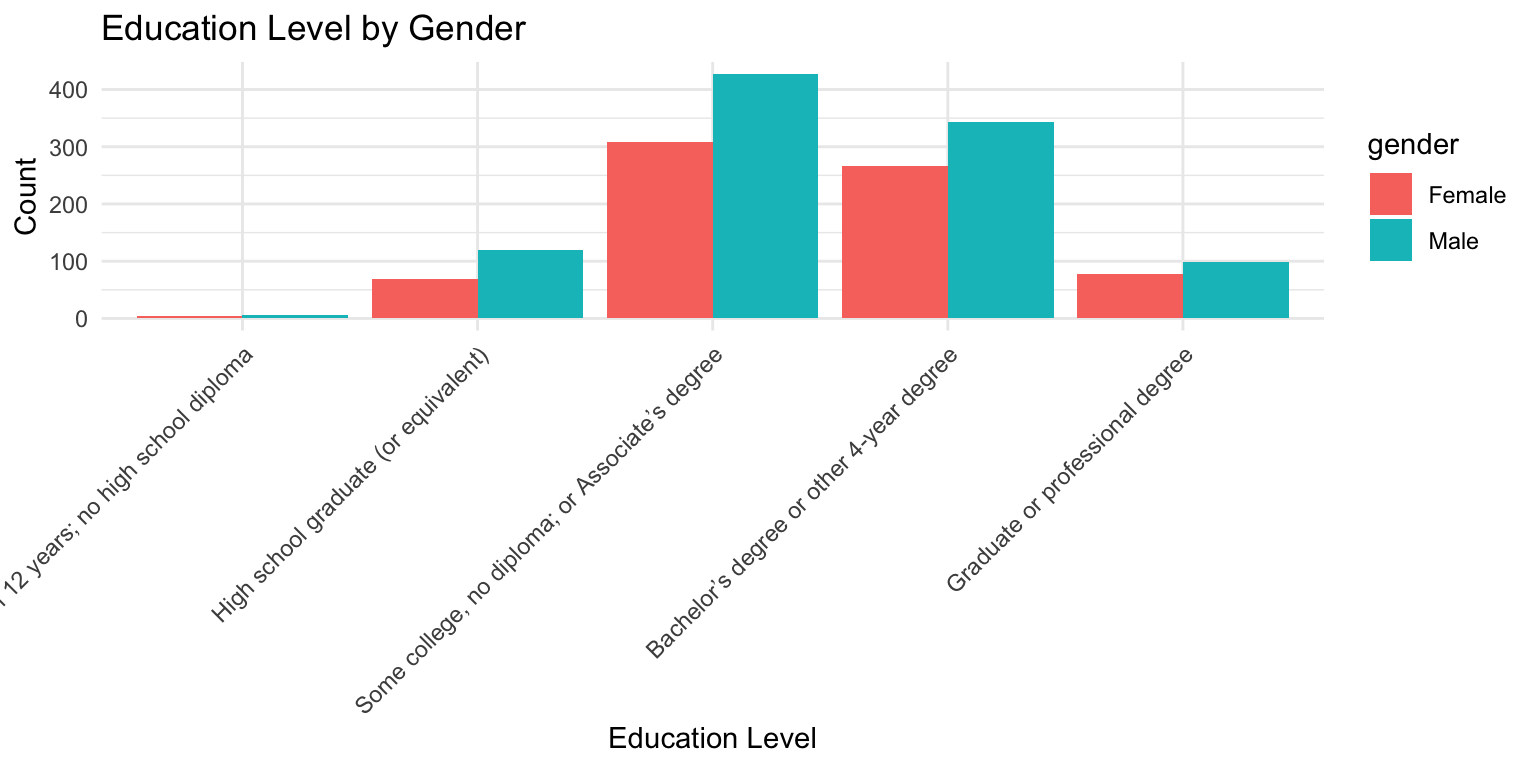
\includegraphics{hw1_sp2024_files/figure-latex/unnamed-chunk-4-1.pdf}
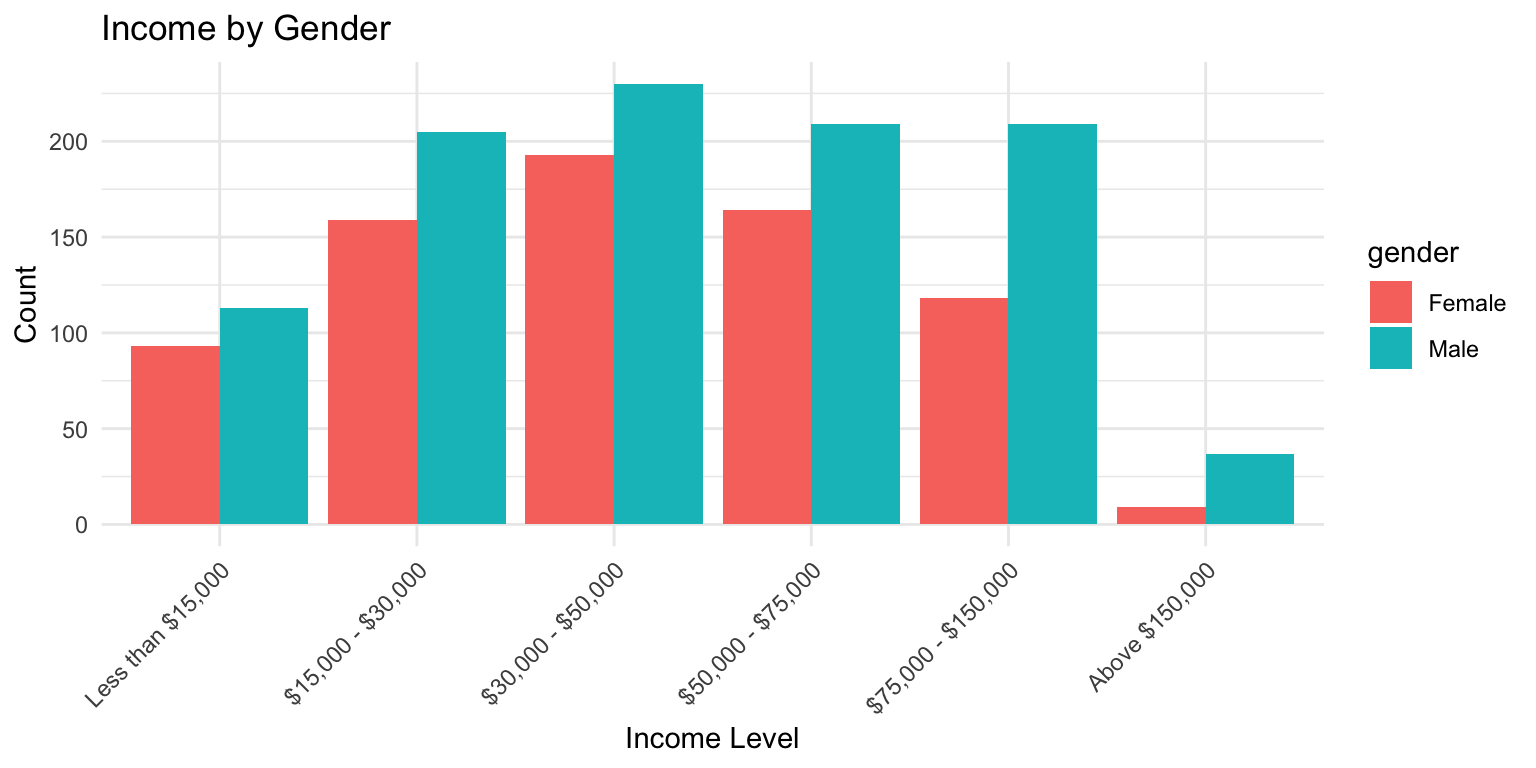
\includegraphics{hw1_sp2024_files/figure-latex/unnamed-chunk-4-2.pdf}
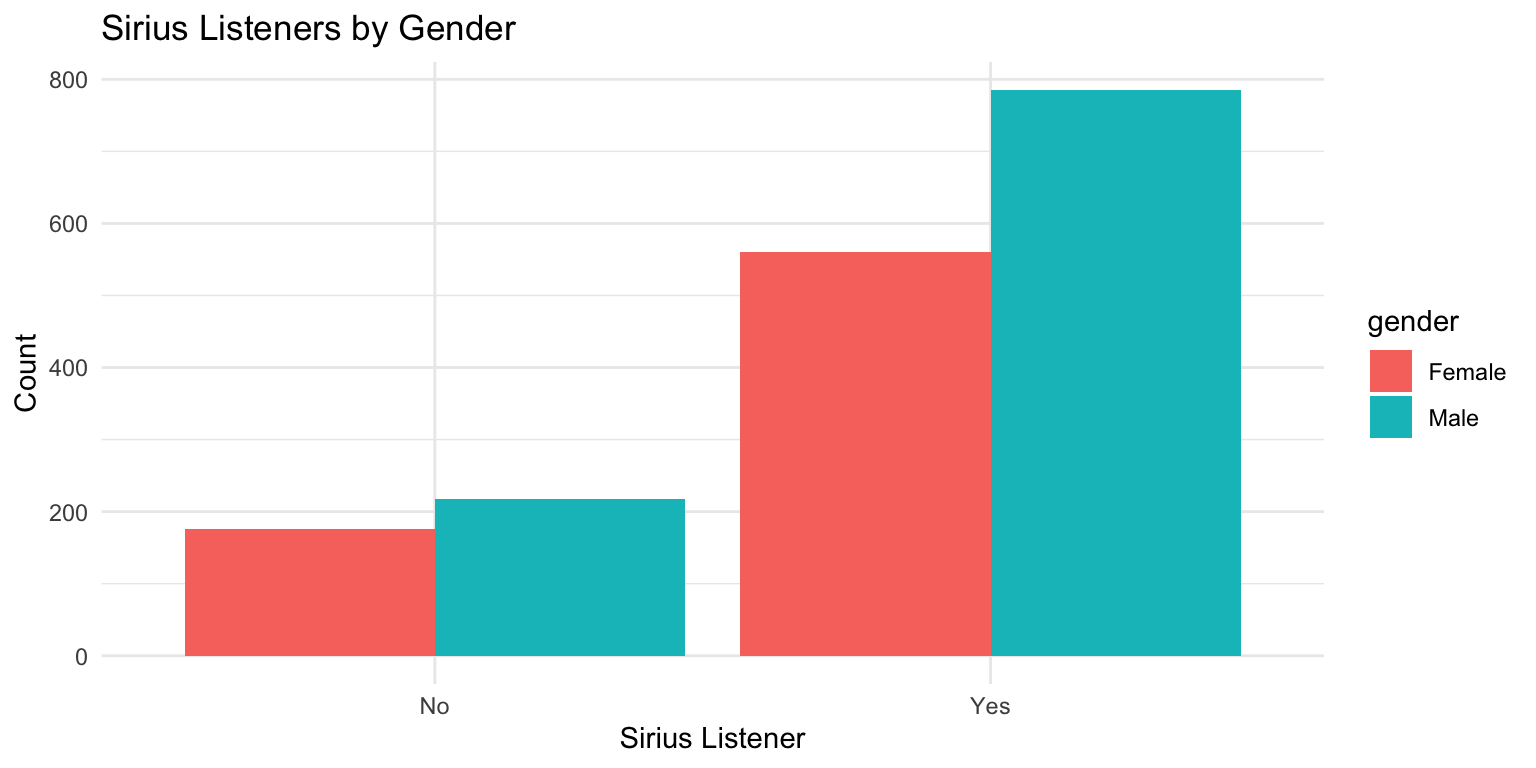
\includegraphics{hw1_sp2024_files/figure-latex/unnamed-chunk-4-3.pdf}
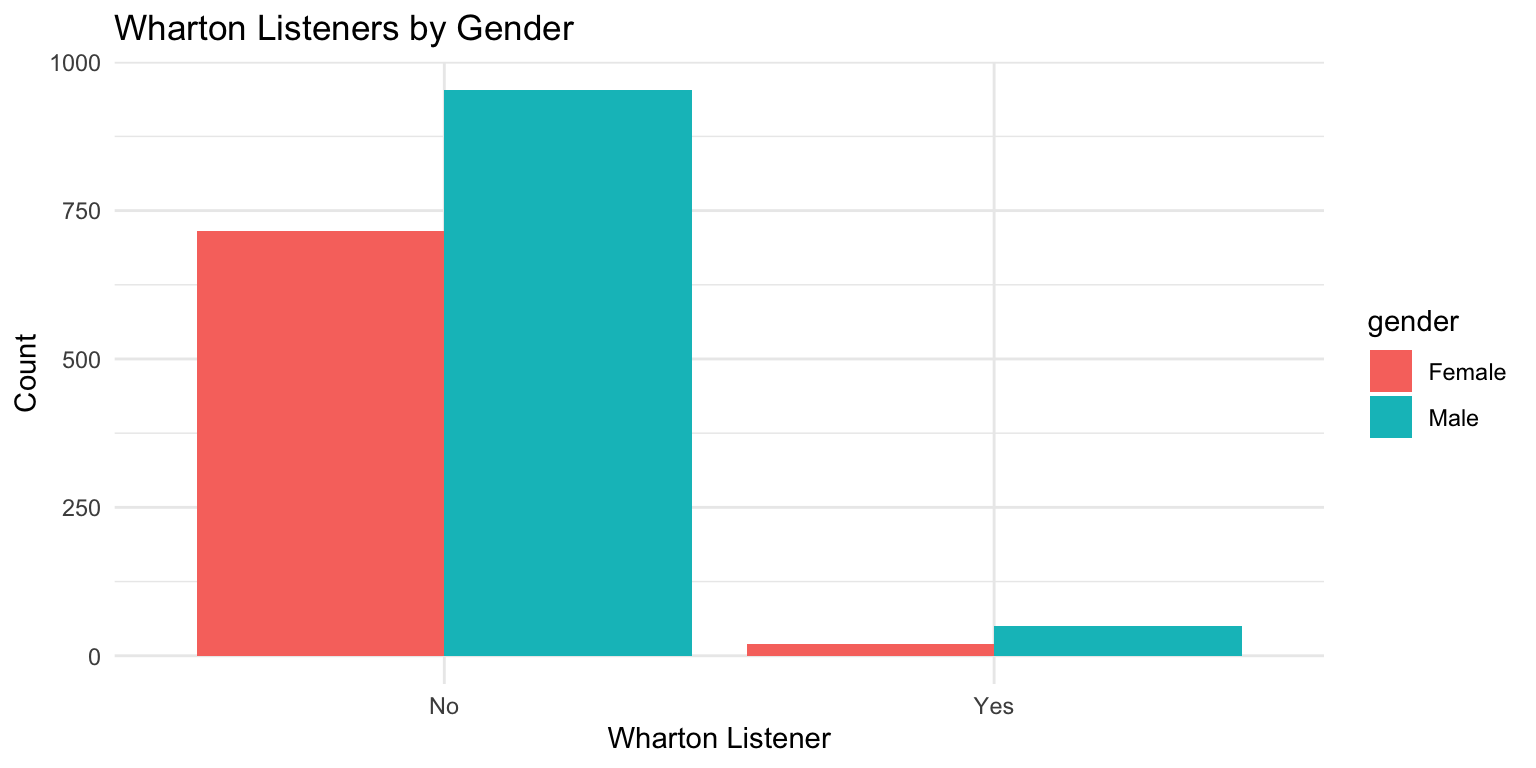
\includegraphics{hw1_sp2024_files/figure-latex/unnamed-chunk-4-4.pdf}
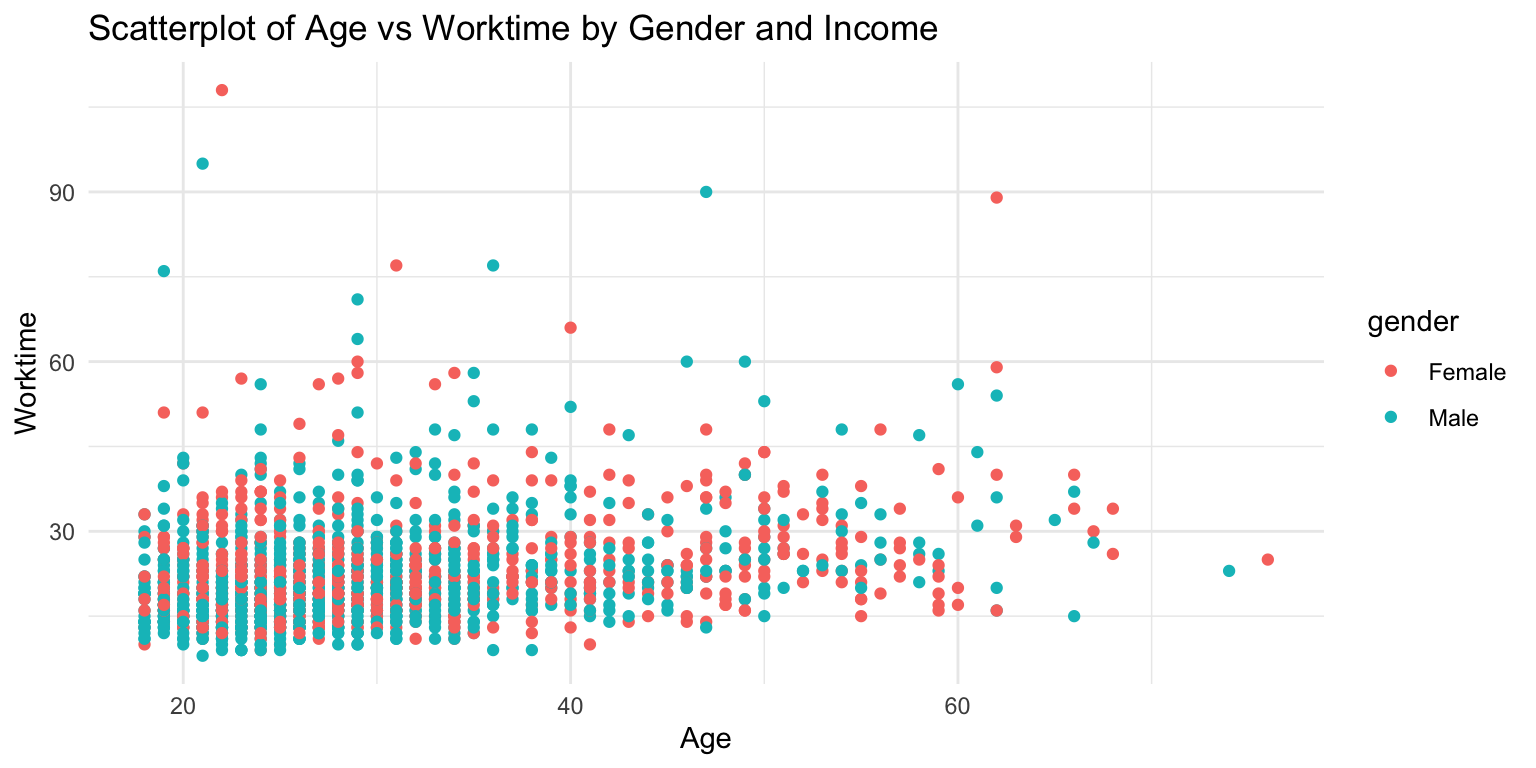
\includegraphics{hw1_sp2024_files/figure-latex/unnamed-chunk-4-5.pdf}

\begin{verbatim}
## Warning in grid.Call(C_textBounds, as.graphicsAnnot(x$label), x$x, x$y, :
## conversion failure on 'Some college, no diploma; or Associate’s degree' in
## 'mbcsToSbcs': dot substituted for <e2>
\end{verbatim}

\begin{verbatim}
## Warning in grid.Call(C_textBounds, as.graphicsAnnot(x$label), x$x, x$y, :
## conversion failure on 'Some college, no diploma; or Associate’s degree' in
## 'mbcsToSbcs': dot substituted for <80>
\end{verbatim}

\begin{verbatim}
## Warning in grid.Call(C_textBounds, as.graphicsAnnot(x$label), x$x, x$y, :
## conversion failure on 'Some college, no diploma; or Associate’s degree' in
## 'mbcsToSbcs': dot substituted for <99>
\end{verbatim}

\begin{verbatim}
## Warning in grid.Call(C_textBounds, as.graphicsAnnot(x$label), x$x, x$y, :
## conversion failure on 'Bachelor’s degree or other 4-year degree' in
## 'mbcsToSbcs': dot substituted for <e2>
\end{verbatim}

\begin{verbatim}
## Warning in grid.Call(C_textBounds, as.graphicsAnnot(x$label), x$x, x$y, :
## conversion failure on 'Bachelor’s degree or other 4-year degree' in
## 'mbcsToSbcs': dot substituted for <80>
\end{verbatim}

\begin{verbatim}
## Warning in grid.Call(C_textBounds, as.graphicsAnnot(x$label), x$x, x$y, :
## conversion failure on 'Bachelor’s degree or other 4-year degree' in
## 'mbcsToSbcs': dot substituted for <99>
\end{verbatim}

\begin{verbatim}
## Warning in grid.Call(C_textBounds, as.graphicsAnnot(x$label), x$x, x$y, :
## conversion failure on 'Some college, no diploma; or Associate’s degree' in
## 'mbcsToSbcs': dot substituted for <e2>
\end{verbatim}

\begin{verbatim}
## Warning in grid.Call(C_textBounds, as.graphicsAnnot(x$label), x$x, x$y, :
## conversion failure on 'Some college, no diploma; or Associate’s degree' in
## 'mbcsToSbcs': dot substituted for <80>
\end{verbatim}

\begin{verbatim}
## Warning in grid.Call(C_textBounds, as.graphicsAnnot(x$label), x$x, x$y, :
## conversion failure on 'Some college, no diploma; or Associate’s degree' in
## 'mbcsToSbcs': dot substituted for <99>
\end{verbatim}

\begin{verbatim}
## Warning in grid.Call(C_textBounds, as.graphicsAnnot(x$label), x$x, x$y, :
## conversion failure on 'Bachelor’s degree or other 4-year degree' in
## 'mbcsToSbcs': dot substituted for <e2>
\end{verbatim}

\begin{verbatim}
## Warning in grid.Call(C_textBounds, as.graphicsAnnot(x$label), x$x, x$y, :
## conversion failure on 'Bachelor’s degree or other 4-year degree' in
## 'mbcsToSbcs': dot substituted for <80>
\end{verbatim}

\begin{verbatim}
## Warning in grid.Call(C_textBounds, as.graphicsAnnot(x$label), x$x, x$y, :
## conversion failure on 'Bachelor’s degree or other 4-year degree' in
## 'mbcsToSbcs': dot substituted for <99>
\end{verbatim}

\begin{verbatim}
## Warning in grid.Call(C_textBounds, as.graphicsAnnot(x$label), x$x, x$y, :
## conversion failure on 'Some college, no diploma; or Associate’s degree' in
## 'mbcsToSbcs': dot substituted for <e2>
\end{verbatim}

\begin{verbatim}
## Warning in grid.Call(C_textBounds, as.graphicsAnnot(x$label), x$x, x$y, :
## conversion failure on 'Some college, no diploma; or Associate’s degree' in
## 'mbcsToSbcs': dot substituted for <80>
\end{verbatim}

\begin{verbatim}
## Warning in grid.Call(C_textBounds, as.graphicsAnnot(x$label), x$x, x$y, :
## conversion failure on 'Some college, no diploma; or Associate’s degree' in
## 'mbcsToSbcs': dot substituted for <99>
\end{verbatim}

\begin{verbatim}
## Warning in grid.Call(C_textBounds, as.graphicsAnnot(x$label), x$x, x$y, :
## conversion failure on 'Bachelor’s degree or other 4-year degree' in
## 'mbcsToSbcs': dot substituted for <e2>
\end{verbatim}

\begin{verbatim}
## Warning in grid.Call(C_textBounds, as.graphicsAnnot(x$label), x$x, x$y, :
## conversion failure on 'Bachelor’s degree or other 4-year degree' in
## 'mbcsToSbcs': dot substituted for <80>
\end{verbatim}

\begin{verbatim}
## Warning in grid.Call(C_textBounds, as.graphicsAnnot(x$label), x$x, x$y, :
## conversion failure on 'Bachelor’s degree or other 4-year degree' in
## 'mbcsToSbcs': dot substituted for <99>
\end{verbatim}

\begin{verbatim}
## Warning in grid.Call(C_textBounds, as.graphicsAnnot(x$label), x$x, x$y, :
## conversion failure on 'Some college, no diploma; or Associate’s degree' in
## 'mbcsToSbcs': dot substituted for <e2>
\end{verbatim}

\begin{verbatim}
## Warning in grid.Call(C_textBounds, as.graphicsAnnot(x$label), x$x, x$y, :
## conversion failure on 'Some college, no diploma; or Associate’s degree' in
## 'mbcsToSbcs': dot substituted for <80>
\end{verbatim}

\begin{verbatim}
## Warning in grid.Call(C_textBounds, as.graphicsAnnot(x$label), x$x, x$y, :
## conversion failure on 'Some college, no diploma; or Associate’s degree' in
## 'mbcsToSbcs': dot substituted for <99>
\end{verbatim}

\begin{verbatim}
## Warning in grid.Call(C_textBounds, as.graphicsAnnot(x$label), x$x, x$y, :
## conversion failure on 'Bachelor’s degree or other 4-year degree' in
## 'mbcsToSbcs': dot substituted for <e2>
\end{verbatim}

\begin{verbatim}
## Warning in grid.Call(C_textBounds, as.graphicsAnnot(x$label), x$x, x$y, :
## conversion failure on 'Bachelor’s degree or other 4-year degree' in
## 'mbcsToSbcs': dot substituted for <80>
\end{verbatim}

\begin{verbatim}
## Warning in grid.Call(C_textBounds, as.graphicsAnnot(x$label), x$x, x$y, :
## conversion failure on 'Bachelor’s degree or other 4-year degree' in
## 'mbcsToSbcs': dot substituted for <99>
\end{verbatim}

\begin{verbatim}
## Warning in grid.Call(C_textBounds, as.graphicsAnnot(x$label), x$x, x$y, :
## conversion failure on 'Some college, no diploma; or Associate’s degree' in
## 'mbcsToSbcs': dot substituted for <e2>
\end{verbatim}

\begin{verbatim}
## Warning in grid.Call(C_textBounds, as.graphicsAnnot(x$label), x$x, x$y, :
## conversion failure on 'Some college, no diploma; or Associate’s degree' in
## 'mbcsToSbcs': dot substituted for <80>
\end{verbatim}

\begin{verbatim}
## Warning in grid.Call(C_textBounds, as.graphicsAnnot(x$label), x$x, x$y, :
## conversion failure on 'Some college, no diploma; or Associate’s degree' in
## 'mbcsToSbcs': dot substituted for <99>
\end{verbatim}

\begin{verbatim}
## Warning in grid.Call(C_textBounds, as.graphicsAnnot(x$label), x$x, x$y, :
## conversion failure on 'Bachelor’s degree or other 4-year degree' in
## 'mbcsToSbcs': dot substituted for <e2>
\end{verbatim}

\begin{verbatim}
## Warning in grid.Call(C_textBounds, as.graphicsAnnot(x$label), x$x, x$y, :
## conversion failure on 'Bachelor’s degree or other 4-year degree' in
## 'mbcsToSbcs': dot substituted for <80>
\end{verbatim}

\begin{verbatim}
## Warning in grid.Call(C_textBounds, as.graphicsAnnot(x$label), x$x, x$y, :
## conversion failure on 'Bachelor’s degree or other 4-year degree' in
## 'mbcsToSbcs': dot substituted for <99>
\end{verbatim}

\begin{verbatim}
## Warning in grid.Call(C_textBounds, as.graphicsAnnot(x$label), x$x, x$y, :
## conversion failure on 'Some college, no diploma; or Associate’s degree' in
## 'mbcsToSbcs': dot substituted for <e2>
\end{verbatim}

\begin{verbatim}
## Warning in grid.Call(C_textBounds, as.graphicsAnnot(x$label), x$x, x$y, :
## conversion failure on 'Some college, no diploma; or Associate’s degree' in
## 'mbcsToSbcs': dot substituted for <80>
\end{verbatim}

\begin{verbatim}
## Warning in grid.Call(C_textBounds, as.graphicsAnnot(x$label), x$x, x$y, :
## conversion failure on 'Some college, no diploma; or Associate’s degree' in
## 'mbcsToSbcs': dot substituted for <99>
\end{verbatim}

\begin{verbatim}
## Warning in grid.Call(C_textBounds, as.graphicsAnnot(x$label), x$x, x$y, :
## conversion failure on 'Bachelor’s degree or other 4-year degree' in
## 'mbcsToSbcs': dot substituted for <e2>
\end{verbatim}

\begin{verbatim}
## Warning in grid.Call(C_textBounds, as.graphicsAnnot(x$label), x$x, x$y, :
## conversion failure on 'Bachelor’s degree or other 4-year degree' in
## 'mbcsToSbcs': dot substituted for <80>
\end{verbatim}

\begin{verbatim}
## Warning in grid.Call(C_textBounds, as.graphicsAnnot(x$label), x$x, x$y, :
## conversion failure on 'Bachelor’s degree or other 4-year degree' in
## 'mbcsToSbcs': dot substituted for <99>
\end{verbatim}

\begin{verbatim}
## Warning in grid.Call(C_textBounds, as.graphicsAnnot(x$label), x$x, x$y, :
## conversion failure on 'Some college, no diploma; or Associate’s degree' in
## 'mbcsToSbcs': dot substituted for <e2>
\end{verbatim}

\begin{verbatim}
## Warning in grid.Call(C_textBounds, as.graphicsAnnot(x$label), x$x, x$y, :
## conversion failure on 'Some college, no diploma; or Associate’s degree' in
## 'mbcsToSbcs': dot substituted for <80>
\end{verbatim}

\begin{verbatim}
## Warning in grid.Call(C_textBounds, as.graphicsAnnot(x$label), x$x, x$y, :
## conversion failure on 'Some college, no diploma; or Associate’s degree' in
## 'mbcsToSbcs': dot substituted for <99>
\end{verbatim}

\begin{verbatim}
## Warning in grid.Call(C_textBounds, as.graphicsAnnot(x$label), x$x, x$y, :
## conversion failure on 'Bachelor’s degree or other 4-year degree' in
## 'mbcsToSbcs': dot substituted for <e2>
\end{verbatim}

\begin{verbatim}
## Warning in grid.Call(C_textBounds, as.graphicsAnnot(x$label), x$x, x$y, :
## conversion failure on 'Bachelor’s degree or other 4-year degree' in
## 'mbcsToSbcs': dot substituted for <80>
\end{verbatim}

\begin{verbatim}
## Warning in grid.Call(C_textBounds, as.graphicsAnnot(x$label), x$x, x$y, :
## conversion failure on 'Bachelor’s degree or other 4-year degree' in
## 'mbcsToSbcs': dot substituted for <99>
\end{verbatim}

\begin{verbatim}
## Warning in grid.Call(C_textBounds, as.graphicsAnnot(x$label), x$x, x$y, :
## conversion failure on 'Some college, no diploma; or Associate’s degree' in
## 'mbcsToSbcs': dot substituted for <e2>
\end{verbatim}

\begin{verbatim}
## Warning in grid.Call(C_textBounds, as.graphicsAnnot(x$label), x$x, x$y, :
## conversion failure on 'Some college, no diploma; or Associate’s degree' in
## 'mbcsToSbcs': dot substituted for <80>
\end{verbatim}

\begin{verbatim}
## Warning in grid.Call(C_textBounds, as.graphicsAnnot(x$label), x$x, x$y, :
## conversion failure on 'Some college, no diploma; or Associate’s degree' in
## 'mbcsToSbcs': dot substituted for <99>
\end{verbatim}

\begin{verbatim}
## Warning in grid.Call(C_textBounds, as.graphicsAnnot(x$label), x$x, x$y, :
## conversion failure on 'Bachelor’s degree or other 4-year degree' in
## 'mbcsToSbcs': dot substituted for <e2>
\end{verbatim}

\begin{verbatim}
## Warning in grid.Call(C_textBounds, as.graphicsAnnot(x$label), x$x, x$y, :
## conversion failure on 'Bachelor’s degree or other 4-year degree' in
## 'mbcsToSbcs': dot substituted for <80>
\end{verbatim}

\begin{verbatim}
## Warning in grid.Call(C_textBounds, as.graphicsAnnot(x$label), x$x, x$y, :
## conversion failure on 'Bachelor’s degree or other 4-year degree' in
## 'mbcsToSbcs': dot substituted for <99>
\end{verbatim}

\begin{verbatim}
## Warning in grid.Call(C_textBounds, as.graphicsAnnot(x$label), x$x, x$y, :
## conversion failure on 'Some college, no diploma; or Associate’s degree' in
## 'mbcsToSbcs': dot substituted for <e2>
\end{verbatim}

\begin{verbatim}
## Warning in grid.Call(C_textBounds, as.graphicsAnnot(x$label), x$x, x$y, :
## conversion failure on 'Some college, no diploma; or Associate’s degree' in
## 'mbcsToSbcs': dot substituted for <80>
\end{verbatim}

\begin{verbatim}
## Warning in grid.Call(C_textBounds, as.graphicsAnnot(x$label), x$x, x$y, :
## conversion failure on 'Some college, no diploma; or Associate’s degree' in
## 'mbcsToSbcs': dot substituted for <99>
\end{verbatim}

\begin{verbatim}
## Warning in grid.Call(C_textBounds, as.graphicsAnnot(x$label), x$x, x$y, :
## conversion failure on 'Bachelor’s degree or other 4-year degree' in
## 'mbcsToSbcs': dot substituted for <e2>
\end{verbatim}

\begin{verbatim}
## Warning in grid.Call(C_textBounds, as.graphicsAnnot(x$label), x$x, x$y, :
## conversion failure on 'Bachelor’s degree or other 4-year degree' in
## 'mbcsToSbcs': dot substituted for <80>
\end{verbatim}

\begin{verbatim}
## Warning in grid.Call(C_textBounds, as.graphicsAnnot(x$label), x$x, x$y, :
## conversion failure on 'Bachelor’s degree or other 4-year degree' in
## 'mbcsToSbcs': dot substituted for <99>
\end{verbatim}

\begin{verbatim}
## Warning in grid.Call(C_textBounds, as.graphicsAnnot(x$label), x$x, x$y, :
## conversion failure on 'Some college, no diploma; or Associate’s degree' in
## 'mbcsToSbcs': dot substituted for <e2>
\end{verbatim}

\begin{verbatim}
## Warning in grid.Call(C_textBounds, as.graphicsAnnot(x$label), x$x, x$y, :
## conversion failure on 'Some college, no diploma; or Associate’s degree' in
## 'mbcsToSbcs': dot substituted for <80>
\end{verbatim}

\begin{verbatim}
## Warning in grid.Call(C_textBounds, as.graphicsAnnot(x$label), x$x, x$y, :
## conversion failure on 'Some college, no diploma; or Associate’s degree' in
## 'mbcsToSbcs': dot substituted for <99>
\end{verbatim}

\begin{verbatim}
## Warning in grid.Call(C_textBounds, as.graphicsAnnot(x$label), x$x, x$y, :
## conversion failure on 'Bachelor’s degree or other 4-year degree' in
## 'mbcsToSbcs': dot substituted for <e2>
\end{verbatim}

\begin{verbatim}
## Warning in grid.Call(C_textBounds, as.graphicsAnnot(x$label), x$x, x$y, :
## conversion failure on 'Bachelor’s degree or other 4-year degree' in
## 'mbcsToSbcs': dot substituted for <80>
\end{verbatim}

\begin{verbatim}
## Warning in grid.Call(C_textBounds, as.graphicsAnnot(x$label), x$x, x$y, :
## conversion failure on 'Bachelor’s degree or other 4-year degree' in
## 'mbcsToSbcs': dot substituted for <99>
\end{verbatim}

\begin{verbatim}
## Warning in grid.Call(C_textBounds, as.graphicsAnnot(x$label), x$x, x$y, :
## conversion failure on 'Some college, no diploma; or Associate’s degree' in
## 'mbcsToSbcs': dot substituted for <e2>
\end{verbatim}

\begin{verbatim}
## Warning in grid.Call(C_textBounds, as.graphicsAnnot(x$label), x$x, x$y, :
## conversion failure on 'Some college, no diploma; or Associate’s degree' in
## 'mbcsToSbcs': dot substituted for <80>
\end{verbatim}

\begin{verbatim}
## Warning in grid.Call(C_textBounds, as.graphicsAnnot(x$label), x$x, x$y, :
## conversion failure on 'Some college, no diploma; or Associate’s degree' in
## 'mbcsToSbcs': dot substituted for <99>
\end{verbatim}

\begin{verbatim}
## Warning in grid.Call(C_textBounds, as.graphicsAnnot(x$label), x$x, x$y, :
## conversion failure on 'Bachelor’s degree or other 4-year degree' in
## 'mbcsToSbcs': dot substituted for <e2>
\end{verbatim}

\begin{verbatim}
## Warning in grid.Call(C_textBounds, as.graphicsAnnot(x$label), x$x, x$y, :
## conversion failure on 'Bachelor’s degree or other 4-year degree' in
## 'mbcsToSbcs': dot substituted for <80>
\end{verbatim}

\begin{verbatim}
## Warning in grid.Call(C_textBounds, as.graphicsAnnot(x$label), x$x, x$y, :
## conversion failure on 'Bachelor’s degree or other 4-year degree' in
## 'mbcsToSbcs': dot substituted for <99>
\end{verbatim}

\begin{verbatim}
## Warning in grid.Call(C_textBounds, as.graphicsAnnot(x$label), x$x, x$y, :
## conversion failure on 'Some college, no diploma; or Associate’s degree' in
## 'mbcsToSbcs': dot substituted for <e2>
\end{verbatim}

\begin{verbatim}
## Warning in grid.Call(C_textBounds, as.graphicsAnnot(x$label), x$x, x$y, :
## conversion failure on 'Some college, no diploma; or Associate’s degree' in
## 'mbcsToSbcs': dot substituted for <80>
\end{verbatim}

\begin{verbatim}
## Warning in grid.Call(C_textBounds, as.graphicsAnnot(x$label), x$x, x$y, :
## conversion failure on 'Some college, no diploma; or Associate’s degree' in
## 'mbcsToSbcs': dot substituted for <99>
\end{verbatim}

\begin{verbatim}
## Warning in grid.Call(C_textBounds, as.graphicsAnnot(x$label), x$x, x$y, :
## conversion failure on 'Bachelor’s degree or other 4-year degree' in
## 'mbcsToSbcs': dot substituted for <e2>
\end{verbatim}

\begin{verbatim}
## Warning in grid.Call(C_textBounds, as.graphicsAnnot(x$label), x$x, x$y, :
## conversion failure on 'Bachelor’s degree or other 4-year degree' in
## 'mbcsToSbcs': dot substituted for <80>
\end{verbatim}

\begin{verbatim}
## Warning in grid.Call(C_textBounds, as.graphicsAnnot(x$label), x$x, x$y, :
## conversion failure on 'Bachelor’s degree or other 4-year degree' in
## 'mbcsToSbcs': dot substituted for <99>
\end{verbatim}

\begin{verbatim}
## Warning in grid.Call(C_textBounds, as.graphicsAnnot(x$label), x$x, x$y, :
## conversion failure on 'Some college, no diploma; or Associate’s degree' in
## 'mbcsToSbcs': dot substituted for <e2>
\end{verbatim}

\begin{verbatim}
## Warning in grid.Call(C_textBounds, as.graphicsAnnot(x$label), x$x, x$y, :
## conversion failure on 'Some college, no diploma; or Associate’s degree' in
## 'mbcsToSbcs': dot substituted for <80>
\end{verbatim}

\begin{verbatim}
## Warning in grid.Call(C_textBounds, as.graphicsAnnot(x$label), x$x, x$y, :
## conversion failure on 'Some college, no diploma; or Associate’s degree' in
## 'mbcsToSbcs': dot substituted for <99>
\end{verbatim}

\begin{verbatim}
## Warning in grid.Call(C_textBounds, as.graphicsAnnot(x$label), x$x, x$y, :
## conversion failure on 'Bachelor’s degree or other 4-year degree' in
## 'mbcsToSbcs': dot substituted for <e2>
\end{verbatim}

\begin{verbatim}
## Warning in grid.Call(C_textBounds, as.graphicsAnnot(x$label), x$x, x$y, :
## conversion failure on 'Bachelor’s degree or other 4-year degree' in
## 'mbcsToSbcs': dot substituted for <80>
\end{verbatim}

\begin{verbatim}
## Warning in grid.Call(C_textBounds, as.graphicsAnnot(x$label), x$x, x$y, :
## conversion failure on 'Bachelor’s degree or other 4-year degree' in
## 'mbcsToSbcs': dot substituted for <99>
\end{verbatim}

\begin{verbatim}
## Warning in grid.Call.graphics(C_text, as.graphicsAnnot(x$label), x$x, x$y, :
## conversion failure on 'Some college, no diploma; or Associate’s degree' in
## 'mbcsToSbcs': dot substituted for <e2>
\end{verbatim}

\begin{verbatim}
## Warning in grid.Call.graphics(C_text, as.graphicsAnnot(x$label), x$x, x$y, :
## conversion failure on 'Some college, no diploma; or Associate’s degree' in
## 'mbcsToSbcs': dot substituted for <80>
\end{verbatim}

\begin{verbatim}
## Warning in grid.Call.graphics(C_text, as.graphicsAnnot(x$label), x$x, x$y, :
## conversion failure on 'Some college, no diploma; or Associate’s degree' in
## 'mbcsToSbcs': dot substituted for <99>
\end{verbatim}

\begin{verbatim}
## Warning in grid.Call.graphics(C_text, as.graphicsAnnot(x$label), x$x, x$y, :
## conversion failure on 'Bachelor’s degree or other 4-year degree' in
## 'mbcsToSbcs': dot substituted for <e2>
\end{verbatim}

\begin{verbatim}
## Warning in grid.Call.graphics(C_text, as.graphicsAnnot(x$label), x$x, x$y, :
## conversion failure on 'Bachelor’s degree or other 4-year degree' in
## 'mbcsToSbcs': dot substituted for <80>
\end{verbatim}

\begin{verbatim}
## Warning in grid.Call.graphics(C_text, as.graphicsAnnot(x$label), x$x, x$y, :
## conversion failure on 'Bachelor’s degree or other 4-year degree' in
## 'mbcsToSbcs': dot substituted for <99>
\end{verbatim}

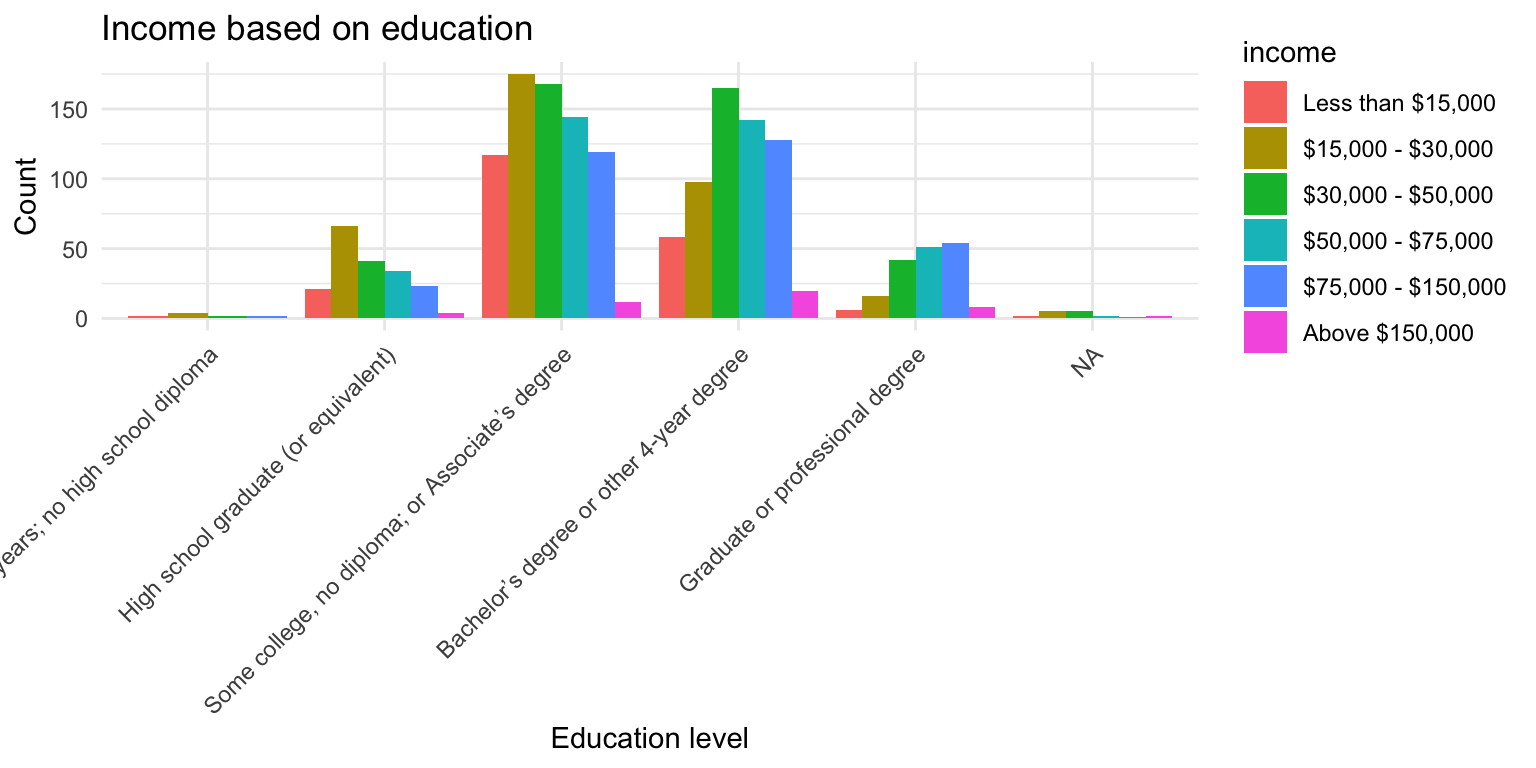
\includegraphics{hw1_sp2024_files/figure-latex/unnamed-chunk-4-6.pdf}

\hypertarget{comments-from-visualizations}{%
\subsubsection{Comments from
visualizations}\label{comments-from-visualizations}}

The education level follows roughly a normal distribution, where most
respondents' education level was some college or a bachelor's degree.
This pattern was the same across both genders.

The income level among females was moreso a normal distribution compared
to that of the men. The females centered around \$30-50k, whereas the
males plateaued from \$15-30k to \$75-150k. Thus, the men are more
represented among the higher income brackets. The mode (i.e.~most
commonly chosen income bracket) was \$30-50k (424 respondents), which
suggests that these survey workers were motivated by the 10 cent
incentive because they have an income lower than the mean household
income in the US.

Additionally, most respondents were Sirius listeners
(\(\frac{1345}{1739}\)) and the majority of the Sirius listeners are
men. Almost all respondents are not Wharton listeners
(\(\frac{70}{1739}\)).

The age of listeners was concentrated around 20 to 40, and worktime was
concentrated under 30 hours. These trends were similar across both
genders. There are some notable outliers, like the 4 year-old
respondent, a 76 year-old respondent and someone with a worktime of 108.

In our income vs education graph, as the education level increases, the
median income level tends to shift from right to left (from lower to
higher income).

\hypertarget{sample-properties}{%
\subsection{Sample properties}\label{sample-properties}}

The population from which the sample is drawn determines where the
results of our analysis can be applied or generalized. We include some
basic demographic information for the purpose of identifying sample
bias, if any exists. Combine our data and the general population
distribution in age, gender and income to try to characterize our sample
on hand.

\begin{enumerate}
\def\labelenumi{\arabic{enumi}.}
\tightlist
\item
  Does this sample appear to be a random sample from the general
  population of the USA? Why it is crucial to have randomness here?
\end{enumerate}

Overall, the data is not very representative of the general US
population.

Our data is majority male (1003 male, 736 female respondents), but the
US population is roughly half male. Additionally, the median age is 28,
but the median age in the US is 38 years-old. The most common income
level is Bachelor's (611), which is representative of about 33\% of the
US population whose highest education level is a Bachelor's. The most
common income level is \$30-50k, which is about \$20-40k lower than the
US average. The average worktime is 21.0 hours, which is considerably
low considering a 9-5 workweek. The vast majority of respondents were
Sirius listeners (\(\frac{1345}{1739}\)), which is not representative
for the overall US population.

Data sources:
\url{https://www.nytimes.com/2023/06/22/us/census-median-age.html},
\url{https://www.census.gov/library/publications/2023/demo/p60-279.html}

It is crucial to have randomness here because if we want to use this
survey to inform how the radio show markets to audiences or use this
data to inform other radio shows, it is crucial to have data that mimics
the overall US.

\begin{enumerate}
\def\labelenumi{\arabic{enumi}.}
\setcounter{enumi}{1}
\tightlist
\item
  Does this sample appear to be a random sample from the MTURK
  population?
\end{enumerate}

Overall, the sample does not appear to be a completely random sample of
the MTURK population. The survey respondents are younger (median 28
years-old) than the MTURK population (median \textasciitilde50-59
years-old). We have majority male (\textasciitilde58\%), whereas MTURK
is majority female (\textasciitilde58\%). The MTURK population has a
higher representation of higher income brackets compared to our data.
For instance, two of the most common income brackets among the MTURK
population is \$50-60k and \$100-150k.

We used the following link for MTURK population demographics data:
(\url{https://www.cloudresearch.com/resources/blog/who-uses-amazon-mturk-2020-demographics/}).

Note: You can not provide evidence by simply looking at our data here.
For example, you need to find distribution of education in our age group
in US to see if the two groups match in distribution. You may need to
gather some background information about the MTURK population to have a
slight sense if this particular sample seem to a random sample from
there\ldots{} Please do not spend too much time gathering evidence.

\hypertarget{final-estimate}{%
\subsection{Final estimate}\label{final-estimate}}

Give a final estimate of the Wharton audience size by May of 2014.
Assume that the sample is a random sample of the MTURK population, and
that the proportion of Wharton listeners vs.~Sirius listeners in the
general population is the same as that in the MTURK population. Write a
brief executive summary to summarize your findings and how you came to
that conclusion.

To be specific, you should include:

\hypertarget{goal-of-the-study}{%
\subsubsection{1. Goal of the study}\label{goal-of-the-study}}

The goal of the study is to estimate the audience size for Wharton
Business Radio on the Sirius radio station using the results from an
MTURK survey of under 2000 respondents in May 2014. We also aimed to
collect demographic information about the survey respondents and see the
relationship between the demographic variables.

\hypertarget{method-used-data-gathering-estimation-methods}{%
\subsubsection{2. Method used: data gathering, estimation
methods}\label{method-used-data-gathering-estimation-methods}}

We used an Amazon MTURK survey to gather data. We then used na.omit() to
clean the data and then removed outliers. We also cleaned the data by
converting to the factor data type to categorize the data. We made
histograms and scatterplots to see the relationship between variables
like education vs.~income. We also used ggplot() and functions like
summary() to visualize and summarize the data.

For estimation methods, we used proportional estimation to predict the
total population. To estimate the total audience size in May 2014, we
multiply the total number of Sirius Radio listeners (given to be 51.6
million) by \(p\), where \(p\) is the proportion of Wharton listeners to
the total number of survey respondents. According to the data summary
above, there are 1348 respondents who listen to Sirius (after filtering
for NAs and outliers), only 70 of which said that they are Wharton
listeners. Thus \(p=\frac{70}{1345}\). So the total number of Wharton
listeners equals 51.6 million times \(\frac{70}{1345}\), which is
2,679,525 Wharton listeners.

\hypertarget{findings}{%
\subsubsection{3. Findings}\label{findings}}

We found based on the above calculations that the estimated number of
Wharton radio listeners is 2,679,525. We also found that the sample was
not completely representiative of the US population or the MTURK
population. Based on the visualizations, we found that the education
level follows roughly a normal distribution, and the income level among
females was moreso a normal distribution compared to that of the men.
The mode (i.e.~most commonly chosen income bracket) was \$30-50k (424
respondents). Also, most respondents were Sirius listeners
(\(\frac{1345}{1739}\)) and the majority of the Sirius listeners are
men. Almost all respondents are not Wharton listeners
(\(\frac{70}{1739}\)).

\hypertarget{limitations-of-the-study.}{%
\subsubsection{4. Limitations of the
study.}\label{limitations-of-the-study.}}

The main limitation of the study was that it was not representative of
the US and MTURK populations. Additionally, the median age is 28, but
the median age in the US is 38 years-old. For instance, we have majority
male (\textasciitilde58\%), whereas MTURK is majority female
(\textasciitilde58\%). Similar differences were seen for the other
variables like education and income. This is a limitation because we
want our survey data to be able to represent the overall populations so
that we can better understand who the radio audience is.

The survey itself is also limited because it does not ask other
information like how often they listen, how long they listen to shows,
how long they have been listening to the radio, etc. The survey could
also collect info on how the respondents would rate their experience
listening to the Wharton Business Radio show and the radio in general.

\hypertarget{new-task}{%
\subsection{New task}\label{new-task}}

We are asked to design a study to estimate the audience size of Wharton
Business Radio Show as of today. We are given a budget of \$1000 and
need to present your findings in two months. Here is our methodology.

\hypertarget{method-proposed-to-estimate-the-audience-size.}{%
\subsubsection{1. Method proposed to estimate the audience
size.}\label{method-proposed-to-estimate-the-audience-size.}}

\hypertarget{survey-platform}{%
\paragraph{Survey Platform:}\label{survey-platform}}

We plan to use the Prolific survey distribution website, which
thoroughly vets its respondents using their IDs. This mitigates the
issue of fake large language model responses that we have observed in
previous surveys using MTurk, which has a lower bar for respondent
entry.

\hypertarget{survey-demographic-filtering}{%
\paragraph{Survey Demographic
Filtering:}\label{survey-demographic-filtering}}

We plan to use Prolific's option of getting a high quality, nationally
representative sample of responses.
\href{https://researcher-help.prolific.com/hc/en-gb/articles/360019236753-Representative-samples\#:~:text=\textquotesingle{}ve\%20tested\%E2\%80\%9D.-,How\%20does\%20Prolific\textquotesingle{}s\%20representative\%20samples\%20tool\%20work\%3F,\%3A\%20age\%2C\%20sex\%20and\%20ethnicity.}{Here
is their article about the feature}, which compares their sample
population with that of the US Census and other large-scale surveys.

\hypertarget{target-sample-size}{%
\paragraph{Target Sample Size:}\label{target-sample-size}}

Given our budget of \$1000, an estimated survey completion time of 1
minute, and a target hourly rate of \$10/hour/respondent, our estimated
maximum number of responses is \(\frac{1000}{10/60}=6000\). We can
iteratively collect and analyze the responses until we have a USA
representative sample size; the representation validity check is
outlined below. By iteratively collecting and analyzing, we can minimize
the costs required to accurately estimate the viewership population.

\hypertarget{data-to-collect}{%
\paragraph{Data to Collect:}\label{data-to-collect}}

\begin{itemize}
\tightlist
\item
  Whether the respondent listens to the Wharton Business Radio Show.
\item
  The respondent's sex.
\item
  The respondent's age.
\item
  The respondent's race.
\end{itemize}

\hypertarget{data-integrity-checks}{%
\paragraph{Data Integrity Checks:}\label{data-integrity-checks}}

After compiling all survey responses, we can 1. Calculate the sex, age,
and race distributions for our 6000 samples. 2. Calculate the sex, age,
and race distributions for the publicly available US Census dataset. 3.
Check if those our sample distributions match that of the US Census. If
not, we may randomly sub-sample our sample dataset to match the
distribution of the broader USA. An example: say our data is skewed
towards an older population than the US census. We may compute the
proportion of the population in each year bracket from the Census data,
then randomly subsample our own dataset to match that distribution. 4.
Compute the proportion of our sample that watches the Wharton Business
Radio Show, and then multiply it by the number of people in the USA to
arrive at our final estimate.

\hypertarget{case-study-2-women-in-science}{%
\section{Case study 2: Women in
Science}\label{case-study-2-women-in-science}}

Are women underrepresented in science in general? How does gender relate
to the type of educational degree pursued? Does the number of higher
degrees increase over the years? In an attempt to answer these
questions, we assembled a data set (\texttt{WomenData\_06\_16.xlsx})
from
\href{https://ncses.nsf.gov/pubs/nsf19304/digest/field-of-degree-women}{NSF}
about various degrees granted in the U.S. from 2006 to 2016. It contains
the following variables: Field (Non-science-engineering
(\texttt{Non-S\&E}) and sciences (\texttt{Computer\ sciences},
\texttt{Mathematics\ and\ statistics}, etc.)), Degree (\texttt{BS},
\texttt{MS}, \texttt{PhD}), Sex (\texttt{M}, \texttt{F}), Number of
degrees granted, and Year.

Our goal is to answer the above questions only through EDA (Exploratory
Data Analyses) without formal testing. We have provided sample R-codes
in the appendix to help you if needed.

\hypertarget{data-preparation-1}{%
\subsection{Data preparation}\label{data-preparation-1}}

\begin{enumerate}
\def\labelenumi{\arabic{enumi}.}
\tightlist
\item
  Understand and clean the data
\end{enumerate}

Notice the data came in as an Excel file. We need to use the package
\texttt{readxl} and the function \texttt{read\_excel()} to read the data
\texttt{WomenData\_06\_16.xlsx} into R.

a). Read the data into R.

b). Clean the names of each variables. (Change variable names to
\texttt{Field},\texttt{Degree}, \texttt{Sex}, \texttt{Year} and
\texttt{Number} )

c). Set the variable natures properly.

d). Any missing values?

There are no missing/NA values.

\begin{enumerate}
\def\labelenumi{\arabic{enumi}.}
\setcounter{enumi}{1}
\tightlist
\item
  Write a summary describing the data set provided here.
\end{enumerate}

a). How many fields are there in this data?

There are 10 fields in this data (printed below).

b). What are the degree types?

There are 3 degree types: BS, MS, PhD.

c). How many year's statistics are being reported here?

There are 11 unique years. (2006 to 2016 contains 11 unique years)

\hypertarget{bs-degrees-in-2015}{%
\subsection{BS degrees in 2015}\label{bs-degrees-in-2015}}

Is there evidence that more males are in science-related fields vs
\texttt{Non-S\&E}? Provide summary statistics and a plot which shows the
number of people by gender and by field. Write a brief summary to
describe your findings.

Yes, there is evidence that there are more males in science related
fields. We provide summary statistics and plots showing gender vs field
in the below analysis, along with a summary of the findings under that.
First, we do some grouping to show the frequency of each gender for each
field in a table:

\begin{verbatim}
## `summarise()` has grouped output by 'Field'. You can override using the
## `.groups` argument.
\end{verbatim}

Based on the plot below which shows the results of the frequency of each
gender for S\&E vs Non S\&E fields, we can see the following:

Visualization 1: Females by far dominate in the Non S\&E category, while
males are slightly more represented when evaluating the S\&E category.
This provides evidence that more males are in science-related fields vs
\texttt{Non-S\&E}.

\begin{verbatim}
## `summarise()` has grouped output by 'SE'. You can override using the `.groups`
## argument.
\end{verbatim}

\includegraphics{hw1_sp2024_files/figure-latex/unnamed-chunk-14-1.pdf}
Based on the plot below, we can see the following:

Visualization 2: Females are the majority (over 60\%) of Non S\&E jobs
pretty consistently across the years, and have been taking an even
greater proportion in recent years (upwards trend in 2014-2016).
However, they are only a smaller fraction of S\&E jobs (below 50\%)
pretty consistently, and have been even less represented in recent years
(downward trend in 2014-2016).

\begin{verbatim}
## `summarise()` has grouped output by 'SE', 'Sex'. You can override using the
## `.groups` argument.
\end{verbatim}

\includegraphics{hw1_sp2024_files/figure-latex/unnamed-chunk-15-1.pdf}

\hypertarget{eda-bringing-type-of-degree-field-and-gender-in-2015}{%
\subsection{EDA bringing type of degree, field and gender in
2015}\label{eda-bringing-type-of-degree-field-and-gender-in-2015}}

Based on the plot below that shows the frequency of each gender for each
field, we can see the following:

Visualization 3: Males are more represented in the computer science and
engineering fields, where as females are more represented in the Non
S\&E fields. Females are higher in fields like psychology and social
science. For instance, in Engineering PhDs, males have 7500 degrees,
whereas females have just 2500 degrees; in contrast, in Non S\&E PhD
degrees, males have just over 10000 degrees whereas females have way
more: 17500 degrees.

\includegraphics{hw1_sp2024_files/figure-latex/unnamed-chunk-16-1.pdf}

Describe the number of people by type of degree, field, and gender. Do
you see any evidence of gender effects over different types of degrees?
Again, provide graphs to summarize your findings.

Based on the plot below that shows the number of people by type of
degree, field, and gender, we can see the following:

Visualization 4: In the BS category for Non S\&E fields, we see an much
steeper upwards trend in females when compared to males, which suggested
there is increasingly more female representation in Non S\&E fields. The
upwards trends for BS in S\&E fields seems relatively alike. In the
masters category, there is a dominance of females in the Non S\&E
fields, whereas for masters in S\&E fields, we see the males
overpowering increasingly, especially in recent years. In the PhD
category, we see very consistent trends over time where females have
more Non S\&E PhDs, where as the males are more in the S\&E PhD
category.

\begin{verbatim}
## `summarise()` has grouped output by 'SE', 'Sex', 'Year'. You can override using
## the `.groups` argument.
\end{verbatim}

\includegraphics{hw1_sp2024_files/figure-latex/unnamed-chunk-17-1.pdf}

Based on the two plots below, we can see the following:

Visualization 5 (Female proportion in SE/non-SE across year by degree):
As the type of degree becomes higher and higher in education level, we
see less ratio of females in S\&E degrees across the years. In recent
years, the gap between the ratio of females in non S\&E jobs and the
ratio of females in S\&E jobs is widening. For instance, in Masters in
S\&E degrees from 2014-2016 we see a downwards trend. The least stable
trend over the years is the ratio of females in Non S\&E PhDs, which has
shown a lot of fluctuation, but shows an upwards trend in recent years.

Visualization 6 (Degrees granted proportion by sex across degree and
SE): We can see that in all of the Non S\&E categories, we have a higher
percentage of females, where as the opposite is true (males dominate,
except for in BS which is almost 50/50 split) in the S\&E categories
across degree type

\begin{verbatim}
## `summarise()` has grouped output by 'SE', 'Sex', 'Year'. You can override using
## the `.groups` argument.
\end{verbatim}

\includegraphics{hw1_sp2024_files/figure-latex/unnamed-chunk-18-1.pdf}

\begin{verbatim}
## `summarise()` has grouped output by 'SE', 'Sex', 'Year'. You can override using
## the `.groups` argument.
\end{verbatim}

\includegraphics{hw1_sp2024_files/figure-latex/unnamed-chunk-19-1.pdf}

\hypertarget{eda-bring-all-variables}{%
\subsection{EDA bring all variables}\label{eda-bring-all-variables}}

In this last portion of the EDA, we ask you to provide evidence
numerically and graphically: Do the number of degrees change by gender,
field, and time?

Visualization 7 and accompanying table: This visualization and the table
brings together all of the variables: number of degrees, gender, field,
and shows the change in these variables over time to analyze how the
number of degrees per field per gender changes every year. We can see a
stronger increase (steeper positive slope) in some of these variables.
For example, in the Non S\&E category, there is a steeper increase in
the number of females with that degree than males (In 2006, Males had
194026, whereas females had 315403. Males in 2016 had 239338 degrees,
Females in 2016 had 393899. We see a greater increase in females with
this degree). We also see in the CS and Engineering fields for the
masters degree, the males have a much greater rate of growth than the
females over time. For some variables, the number of degrees don't
change much over time in terms of gender and field, such as many of the
PhD fields (agricultural science, CS, Non S\&E, etc.). The strongest
increases/changes can be seen in categories like CS and Engineering for
Males in the BS type degree, whereas the increase in females for that
degree is much less steep and looks rather flat. These are some of the
trends we see in this final EDA where we compare all variables over time
form 2006 to 2016.

\includegraphics{hw1_sp2024_files/figure-latex/unnamed-chunk-21-1.pdf}

\hypertarget{women-in-data-science}{%
\subsection{Women in Data Science}\label{women-in-data-science}}

Finally, is there evidence showing that women are underrepresented in
data science? Data science is an interdisciplinary field of computer
science, math, and statistics. You may include year and/or degree.

Visualization 8: We included both year and degree in our chart. We see
that there are significantly more males in the first row (computer
science) as well as in the second row (math/stats). For example, the BS
in CS in 2016 shows over 50000 males and only 10000 females. This
underrepresentation seems to be exacerbated in recent years, as the
number of males in these two fields is increasing more rapidly than the
number of females. The greatest degree of underrepresentation is seen in
the BS and MS categories for the CS field. This underrepresentation is
also seen in the PhD categories for both CS and math/stats.

\includegraphics{hw1_sp2024_files/figure-latex/unnamed-chunk-22-1.pdf}

\hypertarget{final-brief-report}{%
\subsection{Final brief report}\label{final-brief-report}}

Summarize your findings focusing on answering the questions regarding if
we see consistent patterns that more males pursue science-related
fields. Any concerns with the data set? How could we improve on the
study?

DATA: The data seen in the study, called \texttt{WomenData\_06\_16.xlsx}
from
\href{https://ncses.nsf.gov/pubs/nsf19304/digest/field-of-degree-women}{NSF}
provides information from the years 2006 to 2016, specifically in the
US. It contains data about the number of degrees in specific fields, for
specific types of degrees (BS, MS, PhD), by gender, and shows these
trends by containing information about the number of degrees granted
across these 11 years.

GOAL OF THE STUDY: The question at hand was to see if women were
underrepresented in certain fields, namely in science/engineering
fields. The analysis explores how there might be different trends in the
types of degrees pursued based on gender over the years.

METHODS: This case study utilizes EDA (Exploratory Data Analysis) to
collect summary statistics (like mean, median, standard deviation,
frequency, etc. across variables). We use grouping to analyze the data,
specifically using factor data-type columns for this analysis. We also
use the year column to analyze trends over time.

FINDINGS: Our analysis found evidence that suggests that women are
indeed underrepresented in S\&E categories over time. The disparity
seems to be increasing rather than diminishing in the recent years. In
higher degree types, such as masters and PhD, we continue to see this
divide where men are more represented in S\&E fields in this degree
type. Over the years, in S\&E fields, we see stronger increases/steeper
positive slopes for men whereas the number of females with those degrees
appears to be considerably more stagnant.

We saw that in all of the Non S\&E categories, we have a higher
percentage of females, where as the opposite is true (males dominate,
except for in BS which is almost 50/50 split) in the S\&E categories
across degree type. Males are more represented in the computer science
and engineering fields, where as females are more represented in the Non
S\&E fields. Females are higher in fields like psychology and social
science. For instance, in Engineering PhDs, males have 7500 degrees,
whereas females have just 2500 degrees; in contrast, in Non S\&E PhD
degrees, males have just over 10000 degrees whereas females have way
more: 17500 degrees.

These trends show that over time, we have seen an increase in males in
science and engineering degrees, such as math and statistics, while
females tend to be underrepresented in these fields especially in higher
degrees such as MS and PhD when analyzing the data over time from 2006
to 2016.

WAYS TO IMPROVE: The data set is actually very fair and minimally biased
in terms of the data collected. There are 330 females and 330 males, and
the number of data points collected per fields are all 66, and the
number of data points collected per degree type was also 220 for each
BS, MS, and PhD. In this way, the data doesn't seem to be skewed one way
or another. The study can be improved by analyzing data over a longer
period of time, and also by collecting more recent data. The data can
include some more variables, such as information about people dropping
out of degrees, and potentially can be extended to analyze salary/pay by
gender based on the degree field/type that the person received. This
might show more robust results and analyses.

\hypertarget{appendix}{%
\subsection{Appendix}\label{appendix}}

To help out, we have included some R-codes here as references. You
should make your own chunks filled with texts going through each items
listed above. Make sure to hide the unnecessary outputs/code etc.

\begin{enumerate}
\def\labelenumi{\arabic{enumi}.}
\item
  Clean data
\item
  A number of sample analyses
\end{enumerate}

\hypertarget{case-study-3-major-league-baseball}{%
\section{Case study 3: Major League
Baseball}\label{case-study-3-major-league-baseball}}

We would like to explore how payroll affects performance among Major
League Baseball teams. The data is prepared in two formats record
payroll, winning numbers/percentage by team from 1998 to 2014.

Here are the datasets:

-\texttt{MLPayData\_Total.csv}: wide format -\texttt{baseball.csv}: long
format

Feel free to use either dataset to address the problems.

\hypertarget{eda-relationship-between-payroll-changes-and-performance}{%
\subsection{EDA: Relationship between payroll changes and
performance}\label{eda-relationship-between-payroll-changes-and-performance}}

Payroll may relate to performance among ML Baseball teams. One possible
argument is that what affects this year's performance is not this year's
payroll, but the amount that payroll increased from last year. Let us
look into this through EDA.

\begin{verbatim}
## Rows: 510 Columns: 5
## -- Column specification --------------------------------------------------------
## Delimiter: ","
## chr (1): team
## dbl (4): year, payroll, win_num, win_pct
## 
## i Use `spec()` to retrieve the full column specification for this data.
## i Specify the column types or set `show_col_types = FALSE` to quiet this message.
\end{verbatim}

Create increment in payroll a). To describe the increment of payroll in
each year there are several possible approaches. Take 2013 as an
example:

\begin{verbatim}
- option 1: diff: payroll_2013 - payroll_2012
- option 2: log diff: log(payroll_2013) - log(payroll_2012)
\end{verbatim}

Explain why the log difference is more appropriate in this setup.

The log difference calculates the percentage change between the two
years, so that we can see the proportional difference instead of the
absolute difference.

b). Create a new variable
\texttt{diff\_log=log(payroll\_2013)\ -\ log(payroll\_2012)}. Hint: use
\texttt{dplyr::lag()} function.

c). Create a long data table including: team, year, diff\_log, win\_pct

\hypertarget{exploratory-questions}{%
\subsection{Exploratory questions}\label{exploratory-questions}}

a). Which five teams had highest increase in their payroll between years
2010 and 2014, inclusive?

By computing the sum of the log increase in payroll from 2010 to 2014
(inclusive), we found the cumulative log difference in payroll
increases. Using this method, we found that the five teams with the
highest increase in their payroll changes were, in descending order: Los
Angeles Dodgers, Washington Nationals, San Diego Padres, Texas Rangers,
and San Francisco Giants.

b). Between 2010 and 2014, inclusive, which team(s) ``improved'' the
most? That is, had the biggest percentage gain in wins?

The Pittsburgh Pirates and the Baltimore Orioles had the greatest win
improvement, followed by the Washington Nationals and Seattle Mariners,
and finally the Kansas City Royals and Los Angeles Angels.

Note that only one team from the top five payroll increase table managed
to make it into the win percentage table. This may suggest that there is
not a strong relationship between the two variables.

\hypertarget{do-log-increases-in-payroll-imply-better-performance}{%
\subsection{Do log increases in payroll imply better
performance?}\label{do-log-increases-in-payroll-imply-better-performance}}

Is there evidence to support the hypothesis that higher increases in
payroll on the log scale lead to increased performance?

Pick up a few statistics, accompanied with some data visualization, to
support your answer.

\begin{verbatim}
## `geom_smooth()` using formula = 'y ~ x'
\end{verbatim}

\includegraphics{hw1_sp2024_files/figure-latex/unnamed-chunk-30-1.pdf}

\begin{verbatim}
## `geom_smooth()` using formula = 'y ~ x'
\end{verbatim}

\includegraphics{hw1_sp2024_files/figure-latex/unnamed-chunk-31-1.pdf}

From the above regression formula, there is a small, positive, and
statistically significant correlation between the log payroll increase
and the win percentage.

\hypertarget{comparison}{%
\subsection{Comparison}\label{comparison}}

Which set of factors are better explaining performance? Yearly payroll
or yearly increase in payroll? What criterion is being used?

\begin{verbatim}
## `geom_smooth()` using formula = 'y ~ x'
\end{verbatim}

\includegraphics{hw1_sp2024_files/figure-latex/unnamed-chunk-33-1.pdf}

Based on the explained variance values for payroll versus the log change
in payroll, in predicting the win percentage, we can say that payroll is
a better predictor. The higher R-squared value in the payroll analysis
suggests that a larger portion of the variance in win percentage is
explained by the payroll amounts, making it a more substantial factor in
determining a team's performance.

\hypertarget{data}{%
\subsubsection{DATA}\label{data}}

We used baseball.csv, which is a data set that contains information
about various baseball teams' payroll and win percentages/win number
across time from 1998 to 2014.

\hypertarget{goalquestion}{%
\subsubsection{GOAL/QUESTION}\label{goalquestion}}

We want to explore the relationship between payroll and win percentage,
versus seeing if analyzing this relationship is better to do when
calculating the difference in payroll between years rather than the
payroll of the current year itself.

\hypertarget{methods}{%
\subsubsection{METHODS}\label{methods}}

We use EDA to analyze the data and the summary of the variables. We also
create a new table column called diff\_log to analyze the difference of
the log of the payroll for each year, which allows us to analyze the
proportional rather than absolute difference between payrolls across the
year. We also make the table long data, since that is better practice
than using wide data.

\hypertarget{findings-1}{%
\subsubsection{FINDINGS}\label{findings-1}}

Using the cumulative log difference, we found that the five teams with
the highest payroll increase were: Los Angeles Dodgers, Washington
Nationals, San Diego Padres, Texas Rangers, and San Francisco Giants.
The following teams had the highest win percentage gain: Pittsburgh
Pirates, Baltimore Orioles, Washington Nationals, Seattle Mariners, and
Kansas City Royals. We found a positive slope for our best line fit in a
scatterplot plotting win percentage against diff\_log of payroll for the
various teams. We also found a positive slope in the best line of fit
for win percentage vs payroll. When comparing yearly payroll vs yearly
increase in payroll, we found that payroll better explained performance
since it had a higher R-squared/Explained Variance factor and the data
points formed a strong linear relationship, whereas the data points in
the payroll increase graph formed more of a cluster-like shape.

\hypertarget{limitations}{%
\subsubsection{LIMITATIONS}\label{limitations}}

Sometimes payroll increase doesn't mean the same thing for all of the
teams. For instance, the NY Yankees are already so good and already have
so much money that an increase in some amount of money would look like a
small percentage increase, whereas that same amount of money would be a
larger percentage for teams with less money to begin with like the
Pittsburgh Pirates. Better teams probably don't need more money to do
well since they are already so good, while worse teams might not be able
to be more competitive even if they did gain more money.

\end{document}
